\section{A brief history of the Cyan Fluorescent Proteins}\label{sec:prior_T-Cer}
The discovery of the green fluorescent protein (GFP) in the jellyfish \textit{Aequorea victoria} \parencite{shimomuraExtractionPurificationProperties1962}, followed by its cloning \parencite{prasherPrimaryStructureAequorea1992} and the demonstration that it could be used as a marker for gene expression \parencite{chalfieGreenFluorescentProtein1994}, opened the way to a vast array of imaging techniques at the core of contemporary biology. A single mutation of the original \textit{Aequorea victoria}  protein, on position 65:S65T, simplified the fluorescent spectrum of the GFP by simplifying its fluorescence spectrum from two excitation peaks to one single peak at 488 nm, with enhanced amplitude \parencite{heimImprovedGreenFluorescence1995}. The structure of this mutant was later solved, revealing that the GFP consisted of a \textbeta-barrel structure, in which amino acids 65,66 and 67 undergo auto-catalytic cyclization of their backbone to form the chromophore of the protein (\cite{ormoCrystalStructureAequorea1996} Fig. \ref{fig:FP_chromo}).
\begin{figure}[ht] %bt!]
    \centering
    \noindent \includegraphics[width=0.6\textwidth]{images/T-Cer/GFP_autocatalytic_cyclisation.pdf}
    \hfill
    \caption{Autocatalytic cyclisation mechanism leading from a short peptide sequence (Serine-Tyrosine-Glycine) to a fluorophore. The mature, excitable chromophore of the GFP is in the anionic form. Figure reproduced from \cite{cannonRedoxSensitiveGreenFluorescent2009}}
    \label{fig:FP_chromo}
\end{figure}
The first Cyan Fluorescent Protein (CFP) was obtained by combining mutation S65T of the GFP with Y66W: replacing the aromatic residue central to the chromophore triad (\cite{heimWavelengthMutationsPosttranslational1994}, Fig. \ref{fig:CFP_isomere}). A few mutations were needed to accommodate the bulk of the bigger tryptophan, leading to the enhanced CFP (ECFP) \parencite{heimWavelengthMutationsPosttranslational1994}. However, the quantum yield of the ECFP remained low. Building on the crystal structure of the ECFP, a series of beneficial mutations were introduced, creating Cerulean \parencite{rizzoImprovedCyanFluorescent2004}. 

\begin{figure}[ht] %bt!]
    \centering
    \noindent \includegraphics[width=0.8\textwidth]{images/T-Cer/CFP_isomeres.pdf}
    \hfill
    \caption{The CFP chromophore, obtained from the Threonine-Tryptophan-Glycine sequence, and its different stereochemical configurations as calculated from Density Function Theory. (a) configuration Z-Z, (b) configuration E-Z, (c) configuration E,Z and (d) configuration E-E. Figure reproduced from \cite{volianiCisTransPhotoisomerizationFluorescentProtein2008}}
    \label{fig:CFP_isomere}
\end{figure}
The first structure of Cerulean, obtained from a crystal grown at acidic pH (\cite{maloXrayStructureCerulean2007}, right panel in Fig. \ref{fig:Cerulean_pH} (a)) revealed that its chromophore adopted the configuration Z,E (Fig. \ref{fig:CFP_isomere} (b)) while the first structure of Cerulean obtained from crystals grown at neutral pH  (\cite{lelimousinIntrinsicDynamicsECFP2009}, left panel in Fig. \ref{fig:Cerulean_pH} (a)) later revealed a chromophore in configuration Z,Z (Fig. \ref{fig:CFP_isomere} (b)), where the chromophore is stabilised by a hydrogen-bond (H-bond) network encompassing S205, E222, anchoring the chromophore by its indole ring and by the carbonyl of S65 (the first amino-acid in the chromophore triad) (Fig. \ref{fig:Cerulean_pH} (b)).  The group of Antoine Royant generated variants to explore possible fluorescence-enhancing mutations. The fluorescence of one such variant, T65A, was particularly sensitive to pH, with a fluorescence pKa between 5.5 and 6.0 (Fig. \ref{supfig:Fluo_T-Cer}) vs 4.7 for Cerulean \parencite{rizzoImprovedCyanFluorescent2004}.  Similar to all GFP-like proteins, T65A adopts a beta-barrel fold, with the chromophore positioned on the central strand (Fig. \ref{fig:overall}). 

\begin{figure}
    \centering
    \includegraphics[width=0.7\textwidth]{images/T-Cer/Overall.pdf}
    \caption{Global view of the structure of the \textbeta-barrel structure of T65A/Twist-Cerulean variant of the Cerulean fluorescent protein. E222 and S205, involved in the H-bond network stabilising the chromophore at physiological pH, are coloured purple. V150 is coloured red and the 7\textsuperscript{th} strand of the \textbeta-barrel structure is coloured orange. }
    \label{fig:overall}
\end{figure}

Without the carbonyl from the threonine side chain in the first position of the chromophore triad, the H-bond network of the chromophore is only anchored by its indole ring (Fig. \ref{fig:Cerulean_pH} (b)). This is a potential explanation for the exacerbated sensitivity to pH of T65A: in its H-bond network, only one side of E222 is mobilised, and the entire network falls apart when E222 is protonated, whereas in Cerulean E222 conserves its H-bond with the side chain of T65, even at lower pH (Fig. \ref{fig:Cerulean_pH} (a), right panel). Once unanchored, the chromophore of T65A is free to de-excite vibrationally by rotation around its methylene bridge and, therefore, less likely to de-excite by emitting a fluorescence photon upon excitation \parencite{gotthardChromophoreIsomerStabilization2017a}. Strikingly, while the chromophore of Cerulean adopts the Z,E configuration at acidic pH (Fig. \ref{fig:Cerulean_pH} (a)) via a rotation around the CG-CB bond of the methylene bridge, the chromophore of T65A adopts the E,Z configuration at lower pH (Fig. \ref{fig:Cerulean_pH} (b)), corresponding to a rotation around the CA2-CB bond of the methylene bridge.
\begin{figure}[H] %hbt!]
    \centering
    \includegraphics[width=\textwidth]{images/T-Cer/Cer-Tcer_pH.pdf}
    \hfill
    \caption{CFPs chromophore configuration at neutral and acidic pH \textbf{(a)} the cerulean fluorescent protein \textbf{(b)} the T-Cer variant. Structures collected and figures prepared by David von Stetten.}
    \label{fig:Cerulean_pH}
\end{figure}

As the pH drops from neutral to acidic, the transition from configuration Z,Z to Z,E for Cerulean, and Z,Z to E,Z for T65A is accompanied by a blue shift of their main UV-vis absorption band (Fig. \ref{fig:pH_TRspectroinsolution}, unpublished data from the team of Hélène Pasquier, Université Paris-Saclay).  When followed by time-resolved UV-vis absorption spectroscopy in solution after the protein at neutral pH (Tris, pH 8.0) is mixed with an acidic pH buffer (sodium acetate, pH 5.0), the isomerisation process occurs over several hours in Cerulean (Fig. \ref{fig:pH_TRspectroinsolution} (a)). In stark difference, the absorption band of T65A blue loses its two peaked structure and blue shifts in 80 ms (Fig. \ref{fig:pH_TRspectroinsolution} (b)) and remains stable afterwards (Fig. \ref{supfig:Fluo_T-Cer}). Its fast isomerisation earned it the nickname 'Twist-Cerulean" (T-Cer).
\begin{figure}[H] %hbt!]
    \centering
        \noindent \includegraphics[width=\textwidth]{images/T-Cer/insolution_spectro_time.pdf}
    \hfill
    \caption{pH-drop-induced isomerization of the chromophore of Cerulean (a) and T-Cer (b), followed by in-solution absorption spectroscopy after the protein in a neutral pH buffer (Tris, pH 8.0) is mixed with an excess of acidic pH buffer (sodium acetate, pH 5.0) using a stopped-flow device. Spectra go from red (0 s) to blue (4h30 for Cerulean and 80 ms for T-Cer). Figure prepared by Helène Pasquier}
    \label{fig:pH_TRspectroinsolution}
\end{figure}
The surroundings of a fluorophore are tightly packed to maximize fluorescence efficiency. It is intriguing that the important configuration change from Z,Z to E,Z can happen so fast in such a cramped space. The configuration switch presumably occurs over a time scale (80 ms), perfectly matching the capability of the emerging TR-SSX beamlines (particularly beamline ID29 at the ESRF).  Further, at acidic pH, the chromophore of T-Cer adopts a configuration (E,Z) that had not previously been observed for tryptophan-based fluorophores, with altered spectroscopic properties which could serve as the backbone for a  pH-sensing fluorescent protein. 

\vspace{10mm}

Therefore, this project aims to structurally characterise the pH-drop-induced switch of from the reference configuration Z,Z to the novel configuration E,Z in T-Cer, on the \textmu s - s time-domain.

\subsection{List of structures}

Throughout the T-Cer project, several X-ray crystallography structures were determined; they are described in Table \ref{tab:structure-list} (at the end of the section), and will be presented in the coming sections. 
\clearpage
\begin{sidewaystable}[h]
    \begin{tabular}{c>{\centering\arraybackslash}p{0.02\linewidth}>{\centering\arraybackslash}p{0.03\linewidth}>{\centering\arraybackslash}p{0.1\linewidth}>{\centering\arraybackslash}p{0.07\linewidth}c>{\centering\arraybackslash}p{0.07\linewidth}>{\centering\arraybackslash}p{0.08\linewidth}>{\centering\arraybackslash}p{0.07\linewidth}>{\centering\arraybackslash}p{0.02\linewidth}>{\centering\arraybackslash}p{0.02\linewidth}>{\centering\arraybackslash}p{0.02\linewidth}}
         \hline
         Name & pH&   time-point (s)&Sample environnement&  temperature&  beamline &  construct&  precipitant &  resolution (\AA)&  \multicolumn{3}{c}{lattice parameters}\\
         \hline
         & &   &&  &  &  &  &  &  a&  b& c\\
         REF& 8&   &MX&  100 K&  ID30B-ESRF&  T-Cer&  PEG&  1.2&  50.9&  62.7& 69.4\\
         2D& 4&   &MX&  100 K&  ID30B-ESRF&  T-Cer&  PEG&  1.3&  51.6&  62.1& 64.6\\
         8D& 4&   &MX&  100 K&  ID30B-ESRF&  T-Cer&  PEG&  1.4&  51.5&  62.0& 64.5\\
         15D& 4&   &MX&  100 K&  ID30B-ESRF&  T-Cer&  PEG&  1.1&  51.3&  59.2& 64.1\\
         30D& 4&   &MX&  100 K&  ID30A3-ESRF&  T-Cer&  PEG&  1.4&  52.2&  62.6& 65.2\\
         REF-TPD-1& 8&   &Tape-drive&  220 K&  P11-DESY&  T-Cer&  PEG&  1.8&  51.7&  62.8& 70.7\\
         760MS-TPD-1& 8&   0.760&Tape-drive&  220 K&  P11-DESY&  T-Cer&  PEG&  1.8&  51.7&  62.8& 70.7\\
         REF-LAMA& 8&   &Fixed-target&  220 K&  P14-2-DESY&  T-Cer&  PEG&  1.7&  51.9&  62.7& 72.4\\
         3S-LAMA& 8&   3&Fixed-target&  220 K&  P14-2-DESY&  T-Cer&  PEG&  2.3&  50.9&  63.2& 66.0\\
         REF-TPD& 8&   &Tape-drive&  220 K&  P11-DESY&  T-Cer&  PEG&  2.0&  52.0&  63.0& 72.6\\
         3S-TPD-Ac& 8&   3&Tape-drive&  220 K&  P11-DESY&  T-Cer&  PEG&  1.9&  52.0&  63.7& 66.8\\
         8S-TPD-Ac& 8&   8&Tape-drive&  220 K&  P11-DESY&  T-Cer&  PEG&  2.1&  52.0&  63.7& 66.8\\
         300MS-TPD-Ci& 8&   0.300&Tape-drive&  220 K&  P11-DESY&  T-Cer&  PEG&  1.9&  52.0&  63.0& 72.6\\
         1S-TPD-Ci& 8&   1&Tape-drive&  220 K&  P11-DESY&  T-Cer&  PEG&  1.9&  52.0&  63.0& 72.6\\
         3S-TPD-Ci& 8&   3&Tape-drive&  220 K&  P11-DESY&  T-Cer&  PEG&  2.1&  52.0&  63.7& 66.8\\
         8S-TPD-Ci& 8&   8&Tape-drive&  220 K&  P11-DESY&  T-Cer&  PEG&  2.1&  52.0&  63.7& 66.8\\
         16S-TPD-Ci& 8&   16&Tape-drive&  220 K&  P11-DESY&  T-Cer&  PEG&  2.1&  52.0&  63.7& 66.8\\
         REF-TPD-ID29 & 8&   &Tape-drive&  220 K&  ID29-ESRF&  T-Cer&  PEG&  2.2&  51.5&  62.5& 71.0\\
         60S-TPD& 8&   60&Tape-drive&  220 K&  ID29-ESRF&  T-Cer&  PEG&  2.4&  53.0&  63.0& 66.0\\
         150S-CT-S& 8&   150&MX&  100 K&  ID23-2-ESRF&  T-Cer-s&  (NH\textsubscript{4})\textsubscript{2}SO\textsubscript{4}&  1.3&  51.9&  62.5& 66.2\\
         180S-RT-S& 8&   180&MX&  220 K&  ID23-2-ESRF&  T-Cer-s&  (NH\textsubscript{4})\textsubscript{2}SO\textsubscript{4}&  2.2&  52.0&  63.7& 67.7\\
         REF-ALD& 8&   &ALD&  220 K&  PXI-SLS&  T-Cer-s&  (NH\textsubscript{4})\textsubscript{2}SO\textsubscript{4}&  2.2&  51.5&  62.5& 70.5\\
         150S-ALD& 8&   150&ALD&  220 K&  PXI-SLS&  T-Cer-s&  (NH\textsubscript{4})\textsubscript{2}SO\textsubscript{4}&  2.5&  51.6&  61.8& 66.2\\
         300S-ALD& 8&   300&ALD&  220 K&  PXI-SLS&  T-Cer-s&  (NH\textsubscript{4})\textsubscript{2}SO\textsubscript{4}&  2.7&  51.5&  61.1& 65.5\\
         8-V150A& 8&   &MX&  100 K&  BM07-ESRF&  T-Cer-s&  (NH\textsubscript{4})\textsubscript{2}SO\textsubscript{4}&  1.1&  51.1&  62.3& 69.4\\
         4-V150A& 4&   &MX&  100 K&  BM07-ESRF&  T-Cer-s&  (NH\textsubscript{4})\textsubscript{2}SO\textsubscript{4}&  1.3&  51.2&  62.6& 70.1\\
         10S-V150A& 8&   &MX&  100 K&  BM07-ESRF&  T-Cer-s&  (NH\textsubscript{4})\textsubscript{2}SO\textsubscript{4}&  1.0&  51.2&  62.4& 69.1\\
         \hline
    \end{tabular}
    \caption{List of structures of T-Cer and T-Cer-s}\label{tab:structure-list}
\end{sidewaystable}

\section{Preparing the TR-SSX experiment with atomic resolution static structures} \label{sec:ageing}
The isomerisation of the chromophore of T-Cer occurs after a pH drop, therefore we can solve structures of the initial state (pH 8.0, chromophore in the configuration Z,Z) and end state (pH 4.0, chromophore in the configuration E,Z) of the reaction by crystallising T-Cer at physiological and acidic pH. Having access to models refined from high-resolution structures for at least the initial and ground state is beneficial when dealing with a mix of species which are difficult to pull apart.  
\subsection{T-Cer at physiological pH}
This is why the reference structure of T-Cer at pH 8.0 (\textbf{REF}, Table \ref{tab:structure-list}) was reproduced with the conditions described in Section \ref{sec:mat_cryst}. In REF, the chromophore adopts the Z,Z configuration and features the T-Cer H-bond network between E222, S205 and the indole ring of the chromophore (Fig. \ref{fig:T-Cer_pH8vs4} (a)). The maxima in UV-vis absorption signature of T-Cer in solution and \textit{in crystallo} are close (maxima at 438 and 460 nm) (Fig. \ref{supfig:pH8_spec}).
\begin{figure}[H] %bt!]
    \centering
        \noindent \includegraphics[width=\textwidth]{images/T-Cer/T-Cer_pH8vs4.png}
    \hfill
    \caption{Characterisation of T-Cer crystallised at pH 8: (a) Overview of the chromophore (CRC) environment in a structure of T-Cer at neutral pH (1.2 \AA\  resolution, 2\(F_{obs} - F_{calc}\) electron density map contoured at 1.0 \textsigma\ level) collected on beamline ID30b, at the ESRF, red dashed lines represent H-bonds. The chromophore adopts the Z,Z configuration, the carboxyl head of E222 is H-bonded to the hydroxyl group of S205. That same hydroxyl is H-bonded to the indole ring of the chromophore. (b) In the first structure of T-Cer solved from a crystal grown at pH 4.0, 2D (1.2 \AA\ resolution), the configuration Z,Z (lime) is fully populated, S205 is H-bonded to the chromophore, but E222 is no longer H-bonded to S205. The electron density on V150 and Y151 is not as well-defined as for nearby amino acids.}
    \label{fig:T-Cer_pH8vs4}
\end{figure}
\subsection{The structure of T-Cer at acidic pH reveals a metastable Z,Z configured chromophore}
Then, to produce an end-state structure, T-Cer was crystallised at pH 4.0 (conditions in Section \ref{sec:mat_cryst}). Here, we expected a high-resolution structure containing the chromophore in the configuration E,Z. Instead, the chromophore in the first structure of T-Cer solved from a crystal grown at acidic pH was in the Z,Z configuration (Table \ref{tab:structure-list}, Fig. \ref{fig:T-Cer_pH8vs4} (b)). 

\vspace{2mm}

The chromophore isomerisation happens over 80 ms in solution. Therefore, it is reasonable to assume that the chromophore of T-Cer would have isomerised into the configuration E,Z almost instantly when the protein sample was mixed with the pH 4.0 mother liquor, and certainly before crystallisation could happen. And yet, the carboxylic head of E222 is rotated by 20 \degree in the pH 4.0 structure, compared to its position in the REF structure, its H-bond with S205 is severed and it is now H-bonded to the N2 atom of the imidazolinone ring of the chromophore instead (Fig. \ref{fig:T-Cer_pH8vs4} (b)). This reconfiguration of the H-bond network reveals that E222 is indeed protonated in the acidic pH structure. 
This project was founded under the hypothesis that the chromophore adopted the configuration Z,Z at physiological pH, and switched to E,Z at acidic pH in 80 ms. Being able to observe a stable chromophore in the Z,Z configuration at pH 4.0 contradicted one of our hypotheses, as it suggested that the configuration of the chromophore was not (only) pH-dependent. 

\subsection{Crystals of T-Cer cryo-cooled at different delays after they appeared reveal a slow build-up of the E,Z configuration over weeks}

The first structure of T-Cer at pH 4.0 was solved from a crystal cryo-cooled two days after it had grown (overnight). Crystals were fished from the same plate several times to reproduce these results. As a result, the structures of T-Cer at pH 4.0 came from crystals cryo-cooled 8, 15 and 30 days after they had grown, the resulting crystal structures are named \(n\)D where \(n\) is the number of days separating crystal growth (usually overnight) and crystal cryo-cooling (trapping the species contained in the crystal at that time). Accordingly, the first structure (represented in Fig. \ref{fig:T-Cer_pH8vs4} (b)) will be referred to as structure 2D. 

To our surprise, structures 15D and 30D contained a mixture of both configuration and the configuration E,Z exclusively, respectively (Fig. \ref{fig:T-Cer_pH8vs4} (b) and (c)). It appeared that the fraction of E,Z configured chromophore was building up in the crystals as they were left in their crystallisation drop (aged).  

\vspace{2mm}

In 8D, the thinning electron density on V150 suggests it has become flexible (Fig. \ref{fig:ageing_struc} (a)). The spike of electron density under the indole ring of the chromophore suggests that a low occupancy population of the E,Z configuration has appeared. Additionally, the electron density around the imidazolinone ring  has broadened, indicating the coexistence of many alternatively confirmed species that cannot be modelled. Accordingly, E222 is further tilted towards the imidazolinone ring, presumably following its movement.

In 15D, a 55/45 mix of configurations Z,Z (green) and E,Z (purple) and their respective networks of alternate conformations can be observed (Fig. \ref{fig:ageing_struc} (b)). In the E,Z configuration, the imidazolinone ring  retreats into the chromophore pocket, presumably to give the indole head of the chromophore some space to isomerise. There is no electron density (or negligible amounts) between the reference and translated conformations of V150. 


It appears that the slow transition of the 7th strand over days/month that controls the isomerisation \textit{in crystallo} as in structure 30D, the chromophore is entirely E,Z configured and the 7\textsuperscript{th} strand is now stable, in its 'opened' position. Q69 has adopted a new configuration, and a stable water molecule stabilises the indole ring of the chromophore (Fig. \ref{fig:ageing_struc} (c)). Upon closer inspection, the position of V150 in structure 2D would clash with the E,Z configuration of the chromophore. In structure 30D, V150 is translated a full 1 Å outward of the chromophore pocket. Nearby amino acids of the 7\textsuperscript{th} strand are also translated outward, to a lesser degree. 
\begin{figure}[H] %bt!]
    \centering
        \noindent \includegraphics[width=\textwidth]{images/T-Cer/ageing_struc.pdf}
    \hfill
    \caption{Ageing of T-Cer crystals grown at pH 4.0 evidenced via structures of T-Cer cryo-cooled at increasing delays after the crystals appeared. 2\(F_{obs} - F_{calc}\) electron density map contoured at 1.0 r.m.s.d, overlaid on the refined models for the Z,Z conformed (green) and E,Z conformed (purple) species present in the crystal. Dashed lines (green or magenta) represent H-bond networks of both species (respectively Z,Z and E,Z conformed) (a) In 8D (1.4 \AA\ resolution), hint of electron density supporting the low occupancy presence of the configuration E,Z can be seen on the chromophore. The chromophore remains mostly in the Z,Z configuration. S205 and E222 are still engaged in the same H-bond network as in 2D. The electron density on V150 has thinned. (b) In 15D (1.1 \AA\ resolution), both the Z,Z and E,Z configurations can be observed for the chromophore, as well as alternate conformations for S205 and E222, and the 7\textsuperscript{th} strand, one is similar to the conformation in 2D (lime, Z,Z configuration, 55 \% occupancy) and one corresponds to the E,Z configuration (purple, 45 \%). In the latter species, the chromophore is supported by a novel H-bond network, where S205 is disengaged and points upwards, E222 is still H-bonded to the N2 atom of the imidazolinone ring, but has rotated 180 \degree. In addition, the region of the 7\textsuperscript{th} strand is pushed back to allow the E,Z configuration of the chromophore to exist, with V150 being translated of a full 1 \AA. Finally, a novel stable water position, H-bonded to the indole ring of the chromophore, occupies the space freed by the retreat of Q69. (c) The chromophore in 30D (1.4 \AA\ resolution) is fully converted, with only the E,Z configuration of the chromophore and its corresponding alternate conformation network (purple) remaining.}
    \label{fig:ageing_struc}
\end{figure}

The study of the build-up of the E,Z configuration over time (dubbed the 'ageing phenomenon') yielded several insights, altering our working hypothesis that the chromophore adopts the Z,Z configuration at physiological pH, and E,Z configuration at low pH. 
\begin{enumerate}
    \item T-Cer crystallises with its chromophore in the Z,Z configuration. 
    \item At acidic pH \textit{in crystallo}, a metastable (\textasciitilde 2 weeks of half-life) species of T-Cer whose chromophore is in the Z,Z configuration (species MZZ, best represented by structure 2D) initially exists.
    \item MZZ can exist because of a slow reorganisation of the chromophore pocket, involving the 7\textsuperscript{th} strand of the \textbeta-barrel. 
\end{enumerate}

This casts doubts on the configuration of the chromophore in the species formed in 80 ms in solution: does the observed blue-shift correspond to a switch from configuration Z,Z to configuration E,Z, or is the chromophore of T-Cer still in the configuration Z,Z at the end of the experiment? 



\subsection{Matching the X-ray structures of T-Cer to spectroscopic intermediates with UV-vis absorption spectroscopy in solution and \textit{in crystallo}.}
In order to answer that question, we needed to bridge the gap between the species present at the end in-solution time-resolved experiment and our structures of ageing T-Cer. First, we needed to characterise the UV-vis absorption spectroscopy signature of T-Cer over pH in a non-time-resolved manner. 
\subsubsection{The UV-vis absorption spectroscopy signature of T-Cer in solution over pH}
Absorption spectra of T-Cer in solution were recorded from pH 8.0 (blue) to 3.0 (red) Fig. \ref{fig:T-Cer_insolution_pH_static}. From pH 8.0 (blue) to 5.5 (yellow-green), the main absorption band of T-Cer's chromophore loses its two-peak structure, and the centre of mass of the peak blue shifts from 438 nm to 436 nm, as in the time-resolved absorption spectroscopy experiment (Fig. \ref{fig:pH_TRspectroinsolution} (b)). The starkest change occurs between pH 5.5 (yellow-green) and 5.0 (orange), where the main absorption band's centre of mass is significantly blue-shifted to 427 nm (an 11 nm shift from that of the reference state). It further blue-shifts to 423 nm at pH 3.5. Then, at pH 3.0, the centre of mass of the peak reaches 410 nm, probably after the chromophore is exposed to the solvent upon acid-induced denaturation of the protein.
\begin{figure}[H] %bt!]
    \centering
        \noindent \includegraphics[width=0.6\textwidth]{images/T-Cer/In_solution_static_T-Cer.pdf}
    \hfill
    \caption{absorption spectra of T-Cer in solution from pH 8.0 (blue) to 3.0 (red). At neutral pH, the absorption spectroscopy spectrum features a main absorbance peak centred around 435 nm and a shoulder around 450 nm. From pH 8.0 to 6.0, this shoulder is progressively lost. From pH 6.5 to 5, the main absorption band blue-shifts to 430 nm. From pH 5 to pH 4, the main absorption band blue-shifts further to 425 nm.}
    \label{fig:T-Cer_insolution_pH_static}
\end{figure}

\subsubsection{The evolution of the \textit{ic}AS spectrum of T-Cer crystals as they 'age'}
Then, \textit{ic}AS spectra were recorded on crystals cryo-cooled at several points during the 'ageing' process to potentially match their spectroscopic signature with those of the time-resolved pH drop spectroscopy experiment and steady pH points. The spectra are named s\(n\)D accordingly.

In s1D (coloured red, Fig. \ref{fig:ageing_spec}) have a wide absorption band centred on 425 nm, with shoulders at 420, 438 and 450 nm  This most likely corresponds to a mix of species, which probably includes the reference stable Z,Z chromophore (responsible for the 438 and 460 nm shoulders). 

In s2D (coloured orange in Fig. \ref{fig:ageing_spec}), the shoulders at 438 nm and 460 nm disappear, blue-shifting the centre of mass to 420 nm. In s3D:s5D (respectively coloured yellow and light-orange in Fig. \ref{fig:ageing_spec}), the shoulder at 410 nm grows, resulting in a further blue shift of the centre of mass of the absorption band. In s9D:s11D (coloured green to teal in Fig. \ref{fig:ageing_spec}), the shoulder at 410 nm disappears, and the entire band red-shifts to 425 nm. Finally, in s15D (coloured blue spectrum in Fig. \ref{fig:ageing_spec}), the centre of mass of the absorption band is further red-shifted to 430 nm, with a shoulder at 460 nm. 

The 410:420 nm species observed for s2D:s5D, corresponding to MZZ, do not match the last spectrum measured 80 ms after the mixing-induced pH drop during the time-resolved spectroscopy experiment in solution, whose absorption is maximal at 438 nm. Neither do they match the UV-vis spectra of T-Cer in solution at pH 4.0, whose absorption band is maximal at 430 nm. s15D much better matches the spectrum of T-Cer in solution at pH 4.0. However, a shoulder at 460 nm, absent in solution, remains in the spectrum of the 15D crystal, perhaps because it contains a mix of configurations Z,Z and E,Z. \textbf{We can retain the hypothesis that the species formed at pH 4.0 in solution exhibits a chromophore in the E,Z configuration.}

\begin{figure}[H] %bt!]
    \centering
        \noindent \includegraphics[width=0.7\textwidth]{images/T-Cer/ageing_spectra.pdf}
    \hfill
    \caption{\textit{in crystallo} absorption spectra of T-Cer crystals at pH4 over time. In a 1D crystal (red curve), the main absorption band of the spectrum is wide, with a main peak at 425 nm, and shoulders at 420, 425, 435 and 450 nm. In a 2D crystal (orange curve), the main peak of the absorption band is now at 425 nm. In a 3D, 4D and 5D crystal (light orange to bright yellow curves), the main absorbance peak is at 425 nm, and the shoulder at 420 nm has increased in relative height. In 9D and 13D crystals (faded yellow and green curves), the absorption band features only one wide peak centred at 430 nm. After two weeks (blue curve), the absorption band features a main peak at 430 nm and a small shoulder at 450 nm.}
    \label{fig:ageing_spec}
\end{figure}

It appears that the crystalline artefact is not the existence of the E,Z configuration, but rather a prohibited movement of the 7\textsuperscript{th} strand, allowing MZZ to exist, and which exhibits a significantly more blue-shifted absorption band. Several hypotheses, including decreased hydration and mechanical hindrance by the presence of crystal packing points and very close monomers, can explain this prohibited dynamics \textit{in crystallo} (discussed in Section \ref{sec:packingartefact}). The rigidity of the 7\textsuperscript{th} strand is particularly unexpected because this strand is dynamic in Cerulean \parencite{lelimousinIntrinsicDynamicsECFP2009}.

Nevertheless, the sequence of structural reconfiguration leading up to the appearance of configuration E,Z during the 'ageing phenomenon' can serve as a putative model for the sequence of events occurring during the switch from configuration Z,Z to E,Z after a pH drop.

Of note, the lattice parameters in \(n\)D are noticeably shrunk compared to that of REF. This is most pronounced for the C-axis of the unit cell, which is 5 \AA\ shorter in \(n\)D Table \ref{tab:structure-list}. 

\subsection{Atomic resolution structures of T-Cer reveal a different conformation of the C-terminus at physiological and acidic pH}

As for the 'mechanical hindrance' hypothesis, the C-terminal \textalpha-helix of T-Cer (non-visible in published structures of Cerulean \parencite{maloXrayStructureCerulean2007, gotthardCapturingBluelightActivated2023}) is conformed differently REF (green) and \(n\)D (cyan) (Fig. \ref{fig:T_Cer_cter}). In \(n\)D (cyan in Fig. \ref{fig:T_Cer_cter}), the c-terminal \textalpha-helix is positioned near Y200 and Y151, two amino acids which are required to move during the translation of the 7\textsuperscript{th} strand (zoomed-in red rectangle in Fig. \ref{fig:T_Cer_cter}). The additional bulk of the helix could prevent the movement of the 7\textsuperscript{th} strand and thereby prohibit chromophore isomerization. In REF, the C-terminus is positioned away from the \textbeta-barrel. 

\vspace{2mm}

Therefore, T-Cer might be more flexible \textit{in crystallo} when the crystals are grown at pH 8.0. We tried to verify this hypothesis by soaking T-Cer crystals grown at pH 8.0 into pH 4.0 mother liquor, but they did not survive the soak. 

\begin{figure}[H] %bt!]
    \centering
        \noindent \includegraphics[width=\textwidth]{images/T-Cer/C-ter_T-Cer.pdf}
    \hfill
    \caption{Comparison of REF (blue) and 2D (green) structures revealing a different conformation of the C-terminus of T-Cer at acidic and neutral pH, which govern the dynamics of the 7th \textbeta sheet of T-Cer. In crystals obtained at neutral pH, the helix is angled at approximately 90 \degree from the \textbeta-barrel of the chromophore. In crystals obtained at pH 4.0, the helix is positioned along the \textbeta-barrel, close to the 7\textsuperscript{th} strand of the barrel. The tip of the helix in 2D comes close to the position of Y200 and Y151. This hinders the flip of Y200 and Y151, which occurs concurrently with the change of conformation of V150.}
    \label{fig:T_Cer_cter}
\end{figure}

\textbf{To assess whether the chromophore of crystals grown at pH 8.0 would switch from configuration Z,Z to configuration E,Z when the pH in the crystal was lowered, we performed a series of TR-SSX experiments, where the state of T-Cer micro-crystals was probed at various delays after they had been mixed with an acidic solution. }

\section{TR-SSX appraisal of the reaction of T-Cer to a mixing-induced pH drop}

The first TR-SSX experiment took place remotely (due to the COVID-19 health crisis) at beamline P11. Microcrystals of T-Cer were produced by the P11, in DESY team using the protocol described in Section \ref{sec:microcrystallisation}, and mixed with a pH 4.0 mother liquor solution using the CFEL tape-drive \parencite{beyerleinMixanddiffuseSerialSynchrotron2017, zielinskiRapidEfficientRoomtemperature2022} (scheme and setup described in Section \ref{sec:presenting_tpd_P11}). 

\subsection{First tape-drive experiment at P11}

Datasets were recorded 67 to 760 ms after mixing (Table \ref{tab:structure-list}) to sample the time regime defined by the time-resolved UV-vis spectroscopy experiment in solution (Section \ref{sec:prior_T-Cer}). Unfortunately, no meaningful difference between reference and time-points could be observed in the electron density, neither by calculating an \(F_{obs}(time\ point) - F_{obs}(reference\mbox{-}state)\) difference map nor by refining the datasets (reference of the experiment (REF-TPD-1 and 760 ms time-point 760MS-P11 are represented in Fig. \ref{fig:tpd1}). Of note the crystalline lattice of REF-TPD-1 is slightly expanded (1 \AA\ on the C-axis, Table \ref{tab:structure-list}) compared to that of REF, which is expected between datasets collected at room temperature (220K) and cryogenic temperature (100K). 

\vspace{2mm}

Several improvements of the experimental scheme were made for the following beamtimes. T-Cer was submitted to limited proteolysis to increase its flexibility \textit{in crystallo} (Section \ref{sec:limited_proteolysis}). Crystals were mixed with 1M pH 4.0 buffer instead of pH 4.0 mother liquor to decrease viscosity and produce an excess of protons after mixing. 

\subsection{Fixed-target LAMA experiment at P14-2 TREXX}\label{sec:T-REXX}

Using the fixed target liquid dispensing setup described in Section \ref{sec:LAMA}, a datasset was recorded three seconds after the microcrystals of T-Cer were shot by a droplet of pH 4.0 sodium acetate (3S-LAMA, \ref{tab:structure-list}), as well as a reference (REF-LAMA).

In 3S-LAMA, the head of E222 is rotated 30 \degree clockwise, also away from the indole ring of the chromophore and H-bonded to the imidazolinone ring  and S205 is tilted towards E222, away from the indole ring of the chromophore (both are coloured in purple in Fig. \ref{fig:T-Cer_TREXX_results} (b)). Additionally, the electron density is lost on the side-chain of Y151. However, the chromophore and the rest of the chromophore pocket are identical (or comparable) in REF-LAMA and 3S-LAMA (Fig. \ref{fig:T-Cer_TREXX_results} (c)). 

\vspace{2mm}

The 3S-LAMA contains the structure of MZZ, where E222 is protonated, but the chromophore is still in the Z,Z configuration because the 7\textsuperscript{th} strand has not moved yet.
\begin{figure}[H] %bt!]
    \centering
        \noindent \includegraphics[width=\textwidth]{images/T-Cer/TREXX_results.pdf}
    \hfill
    \caption{Results of the T-REXX beamtimes : \(2F_{obs} - F_{calc}\) electron density map contoured at 1.5 \textsigma\ level (a) REF-LAMA (1.7 \AA\ resolution) features a well-defined V150, Y151 as well as an engaged S205 and E222, and Z,Z chromophore. (b) 3S-LAMA (2.3 \AA\ resolution) where Y151 and V150 have flexible side-chains. S205 is tilted upwards, and E222 is disengaged (30 \degree clockwise rotation). These signs suggest that the pH drop has occurred, but the isomerization has not. (c) Superposition of the atomic models of REF-LAMA (cyan) and 3S-LAMA (purple) revealing the difference in orientation of S205 and E222.}\label{fig:T-Cer_TREXX_results}
\end{figure}

\subsection{Second tape-drive mixing experiment at P11}\label{sec:P11-2}

Microcrystals were mixed with 1M pH 4.0 buffer using the fast mixing nozzle of the CFEL tape drive (setup described in Section \ref{sec:presenting_tpd_P11}). Both sodium acetate (Section \ref{sec:acetate}) and sodium citrate (Section \ref{sec:citrate}) were trialled. 

\subsubsection{Sodium acetate}\label{sec:acetate}
Time points were recorded 3 s (3S-TPD-Ac) and 8 s (8S-TPD-Ac) after the crystals were mixed with sodium acetate to validate the reproducibility of the results obtained at T-REXX and further explore the timeline. The reference state of this experiment, REF-TPD, is equivalent to REF-LAMA.

3S-TPD-Ac closely resembles 3S-LAMA (rotated carboxylic head of E222 and tilt of S205, (Fig. \ref{fig:T-Cer_P11-2_Ac_results} (b)). In 8S-TPD-Ac, V150 becomes slightly dynamic (Fig. \ref{fig:T-Cer_P11-2_Ac_results} (c)), but S205 seems to have returned to its initial position (only the model of 3S-TPD-Ac, coloured purple, differs from REF-TPD in Fig. \ref{fig:T-Cer_P11-2_Ac_results} (d)). It is clear that both 3S-TPD-Ac and 8S-TPD-Ac match the structure of MZZ. 
\begin{figure}[H] %bt!]
    \centering
        \noindent 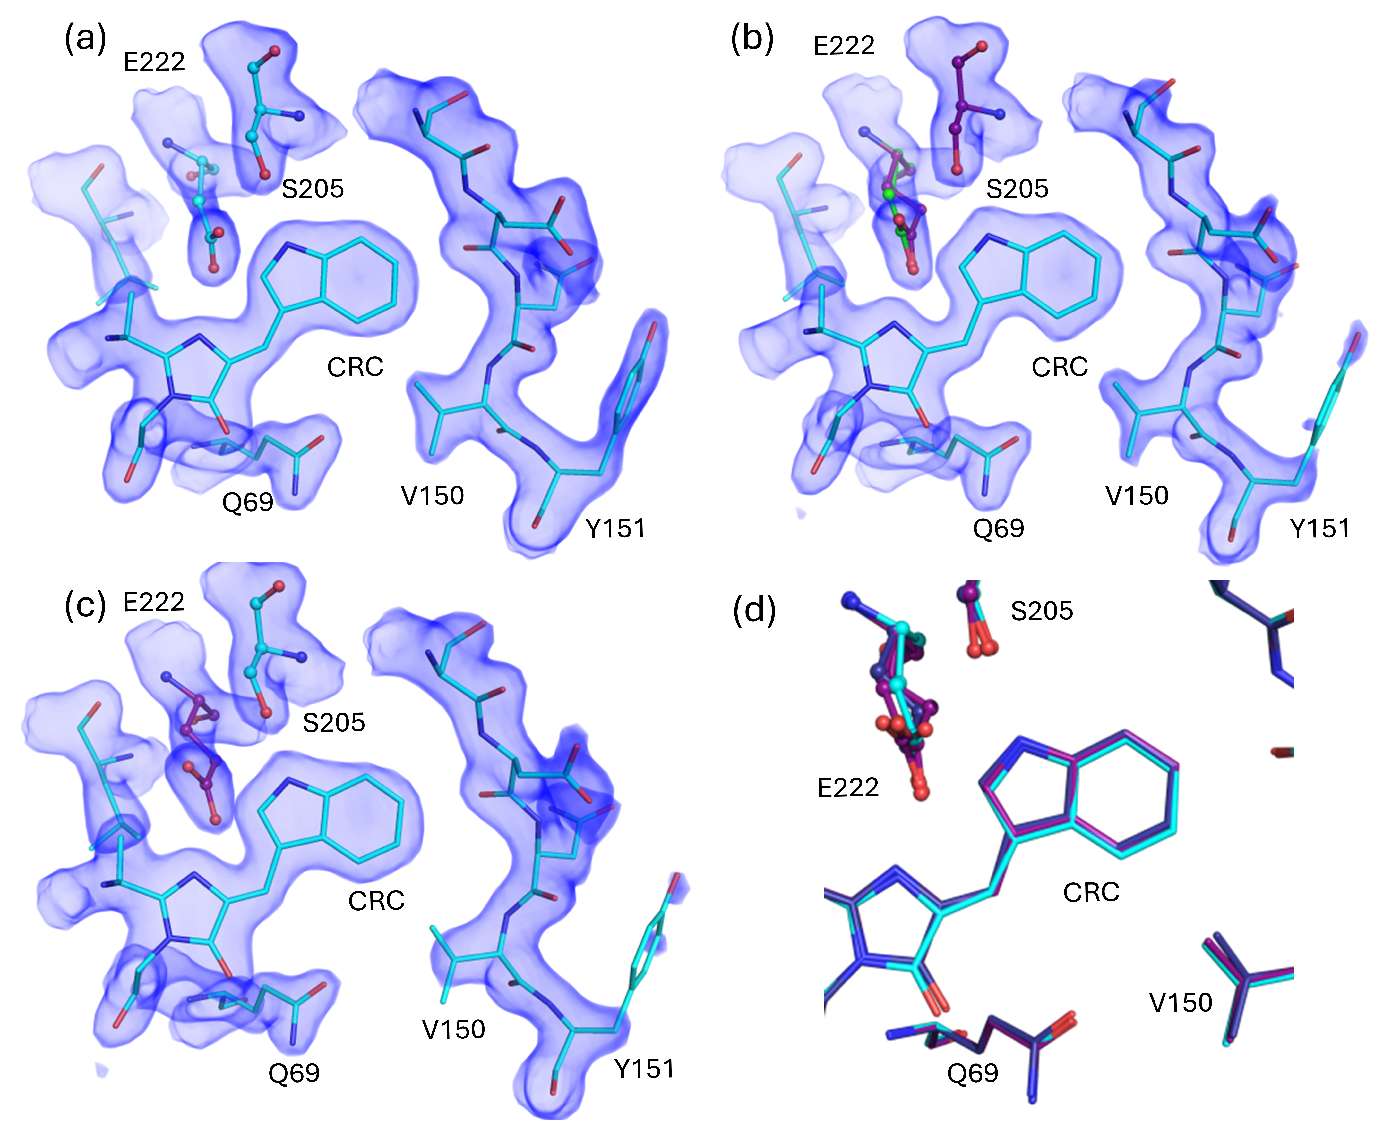
\includegraphics[width=\textwidth]{images/T-Cer/T-Cer_tpd_P11-2_acetate.pdf}
    \hfill
    \caption{Structures of T-Cer after a pH drop induced by mixing with Sodium acetate, 2\(F_{obs} - F_{calc}\) electron density maps contoured at 1.0 \textsigma\ level (a) REF-TPD (2.0 \AA\ resolution) featuring a well-defined V150, Y151 as well as an engaged S205 and E222, and Z,Z chromophore. (b) 3S-TPD-Ac (1.9 \AA\ resolution) S205 (purple) is tilted away from the chromophore. E222 exists in two conformations (green and purple), which are both rotated away from the chromophore. The electron density on Y151 is less defined.  (c) 8S-TPD-Ac (2.2 \AA\ resolution) S205 is back to its initial conformation (coloured in cyan). E222 is fully rotated away from the chromophore (coloured in purple). V150 and Y151 have lost stability. (d) Superposition of refined models for REF-TPD (cyan), 3S-TPD-Ac (purple) and 8S-TPD-Ac (blue), showing the progressive rotation of E222 away from the chromophore and the tilt of S205 at 3s. V150 and nearby amino acids are backing away from the chromophore.: }\label{fig:T-Cer_P11-2_Ac_results}
\end{figure}


\subsubsection{Sodium citrate}\label{sec:citrate}
Time points were recorded 300 ms (300MS-TPD-Ci) and 1 s (1S-TPD-Ci) after mixing  as comparison points with the results of the first beamtime (Supplementary section \ref{sec:P11-1}).  Time points recorded 3 s (3S-TPD-Ci) and 8 s (8S-TPD-Ci) after the crystals were mixed with sodium citrate to serve as comparison points were found to be identical to 3S-TPD-Ac and 8S-TPD-Ac. A last time-point was recorded 16 s after mixing (16S-TPD-Ci) to sample the long-term dynamics of the chromophore. 

In 300MS-TPD-Ci, E222 exists in two conformations (Fig. \ref{fig:T-Cer_P11-2_Ci_results} (a)), which are both rotated away from S205. One is H-bonded to the imidazolinone ring  of the chromophore (MZZ-like, purple) and one is H-bonded to a stable water molecule (not represented) positioned in the background of Fig. \ref{fig:T-Cer_P11-2_Ci_results} (a) (cyan). From 1S-TPD-Ci to 16S-TPD-Ci (Fig. \ref{fig:T-Cer_P11-2_Ci_results} (b) and (c)), only the MZZ-like conformation of E222 remains. 
\begin{figure}[H] %bt!]
    \centering
        \noindent 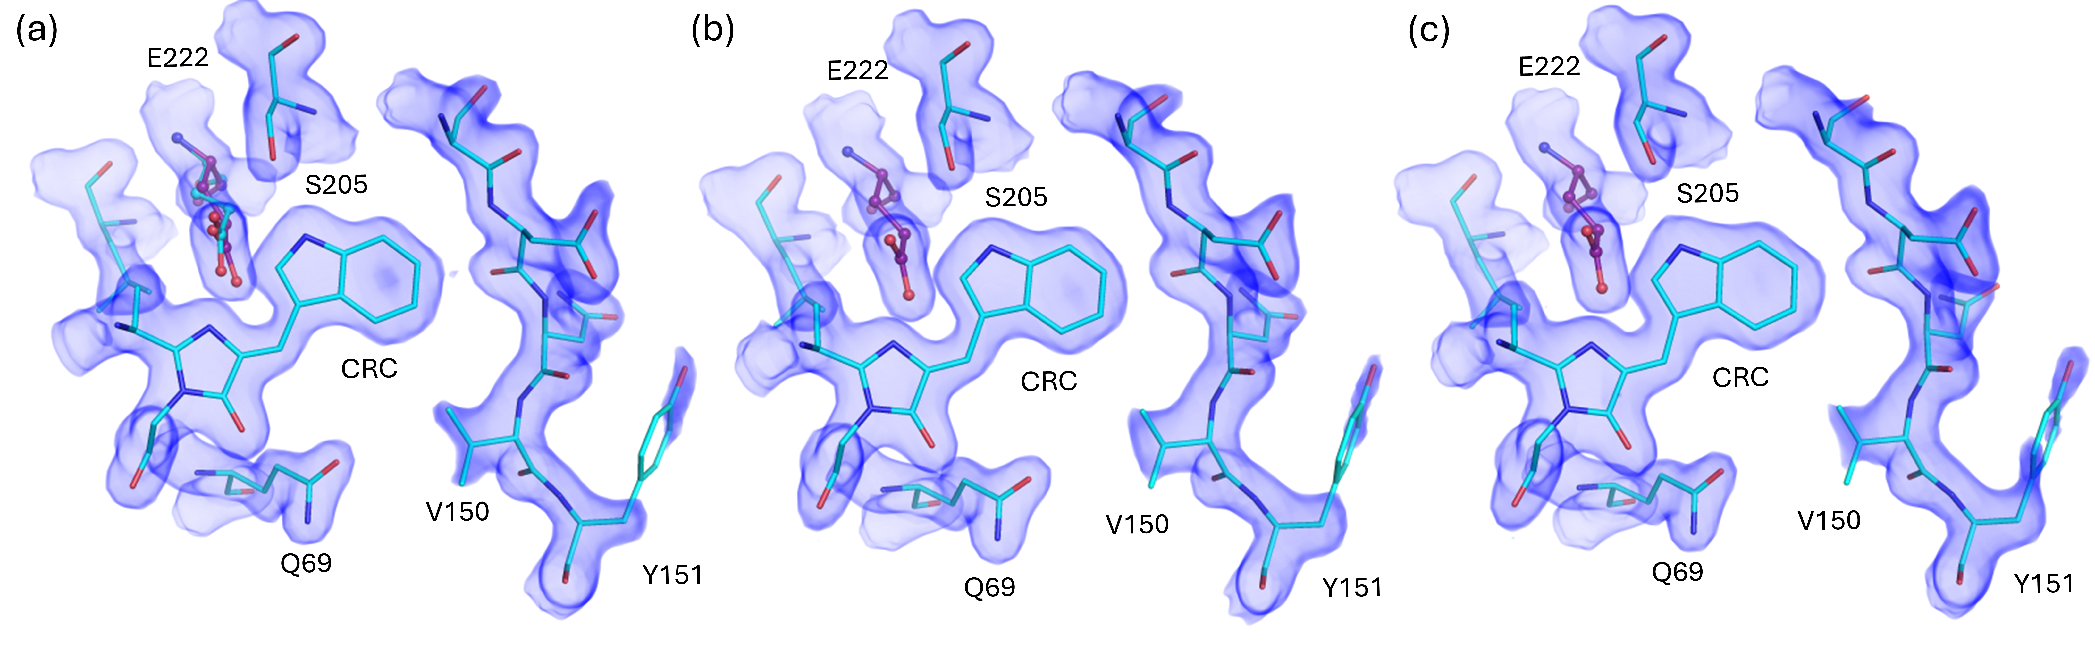
\includegraphics[width=\textwidth]{images/T-Cer/T-Cer_tpd_P11-2_citrate.pdf}
    \hfill
    \caption{Structures of T-Cer after a pH drop induced by mixing with Sodium citrate. All 2\(F_{obs} - F_{calc}\) electron density maps are contoured at 1.0 \textsigma\ level (a) In 300MS-TPD-Ci (1.9 \AA\ resolution), E222 exists in two conformations, which are both rotated away from the chromophore. The electronic density on V150 is still well-defined, but that of Y151 is slightly less defined.  (b) In 1S-TPD-Ci (1.9 \AA\ resolution), E222 is fully rotated away from the chromophore. The side chains of V150 and Y 151 are only partially covered by electron density. (c)  In 16S-TPD-Ci (2.1 \AA\ resolution), E222 is fully rotated away from the chromophore. The side chains of V150 and Y 151 are well covered by electron density, but their strand has moved 0.1 \AA\ away from the chromophore.}\label{fig:T-Cer_P11-2_Ci_results}
\end{figure}

\subsubsection{Discussion of the results produced in TR-SSX beamtimes}\label{sec:discussion_P11_2}

While it has not fully stabilised in the MZZ-like conformation yet, E222 is likely protonated in 300MS-TPD-Ci (Fig. \ref{fig:T-Cer_P11-2_Ci_results} (a)). In comparison, the H-bond between S205 and E222 is intact in 760MS-TPD-1 (Supplementary figure \ref{fig:tpd1} (b)).  Consequences of a pH drop could be observed this time in the ms time-domain, while it they could not in the first beamtime. \textbf{The limited proteolysis step and use of 1M pH buffer succeeded in increasing the flexibility of T-Cer \textit{in crystallo} and/or decreasing the diffusion time of protons in the crystal.}

\vspace{2mm}

Thanks to these advances, the diffusion of protons in the crystals occurs on almost the same time scale as the configuration switch in solution, which would make a TR-SSX able to monitor the mechanism of transition from configuration Z,Z to E,Z after a pH drop. However, despite this advance, all datasets recorded past 300 ms contain a species akin to MZZ, whose chromophore is still in the Z,Z configuration. A trend corresponding to a slight outward translation of V150 (0.1 \AA\ at most) over time can be sighted when modelled from the recorded time points (Fig. \ref{fig:T-Cer_P11-2_Ac_results}), but the system seems stuck in the MZZ state, blocked by the rigidity of the 7\textsuperscript{th} strand.

We can therefore answer some of the questions raised previously. Even in crystals of T-Cer grown at pH 8.0, the packing of T-Cer crystals is clearly inhibiting the movements of the 7\textsuperscript{th} strand, which are needed for the configuration switch. We cannot discern the mechanism underlying the fast switch from configuration Z,Z to E,Z with TR-MX, because even if the isomerisation was to occur \textit{in crystallo}, we could only observe metastable species, and not the reaction intermediate leading from one to another. Finally, our best model so far for this transition is the sequence of events occurring during the ageing phenomenon, which allowed us to observe some of these metastable species. 

Nevertheless, the early response of T-Cer \textit{in crystallo} to a pH drop is now characterised. T-Cer can serve as a commissioning tool for mixing-based TR-SSX setups. 

\section{Commissioning of a Tape-drive setup on ID29}\label{sec:ID29}

In September 2022, beamline ID29 (described in Section \ref{sec:presenting_ID29} was commissioned. During the first beamtime involving external users, T-Cer was used as a commissioning target for a novel tape drive setup (described in Section \ref{sec:lubeck}), as part of an ongoing collaboration with the group of Manfred Roessle in Lubeck. Microcrystals of proteolyzed T-Cer (prepared with the protocol described in Section \ref{sec:limited_proteolysis} and \ref{sec:microcrystallisation}) were mixed with 1 M pH 4.0 sodium citrate via a T-junction and exposed to the beam of ID29 60 s (60S-TPD) later. This was the first genuine TR-MX experiment of the beamline.

In 60S-TPD, E222 adopts the characteristic rotated MZZ-like conformation (Fig. \ref{fig:ID29_results} (b)), the expected reaction to a pH drop, which validates the mixing capabilities of this tape-drive setup. 

\vspace{2mm}

Additionally, S205 and Y151 appear to be dynamic (no longer covered by electron density). Finally, V150 has backed away by 0.3 \AA\ (Fig. \ref{fig:ID29_results} (c)). The movement of the 7\textsuperscript{th} strand has started in 60S-TPD: it is in a more advanced state than in 16S-TPD-Ci. This is coherent with the increased mixing-exposure delay and confirms that, \textit{in crystallo}, T-Cer keeps evolving very slowly over time after a pH drop. 
Whether the isomerisation can happen after a pH drop remains uncertain, however.
\begin{figure}[H] 
    \centering
        \noindent 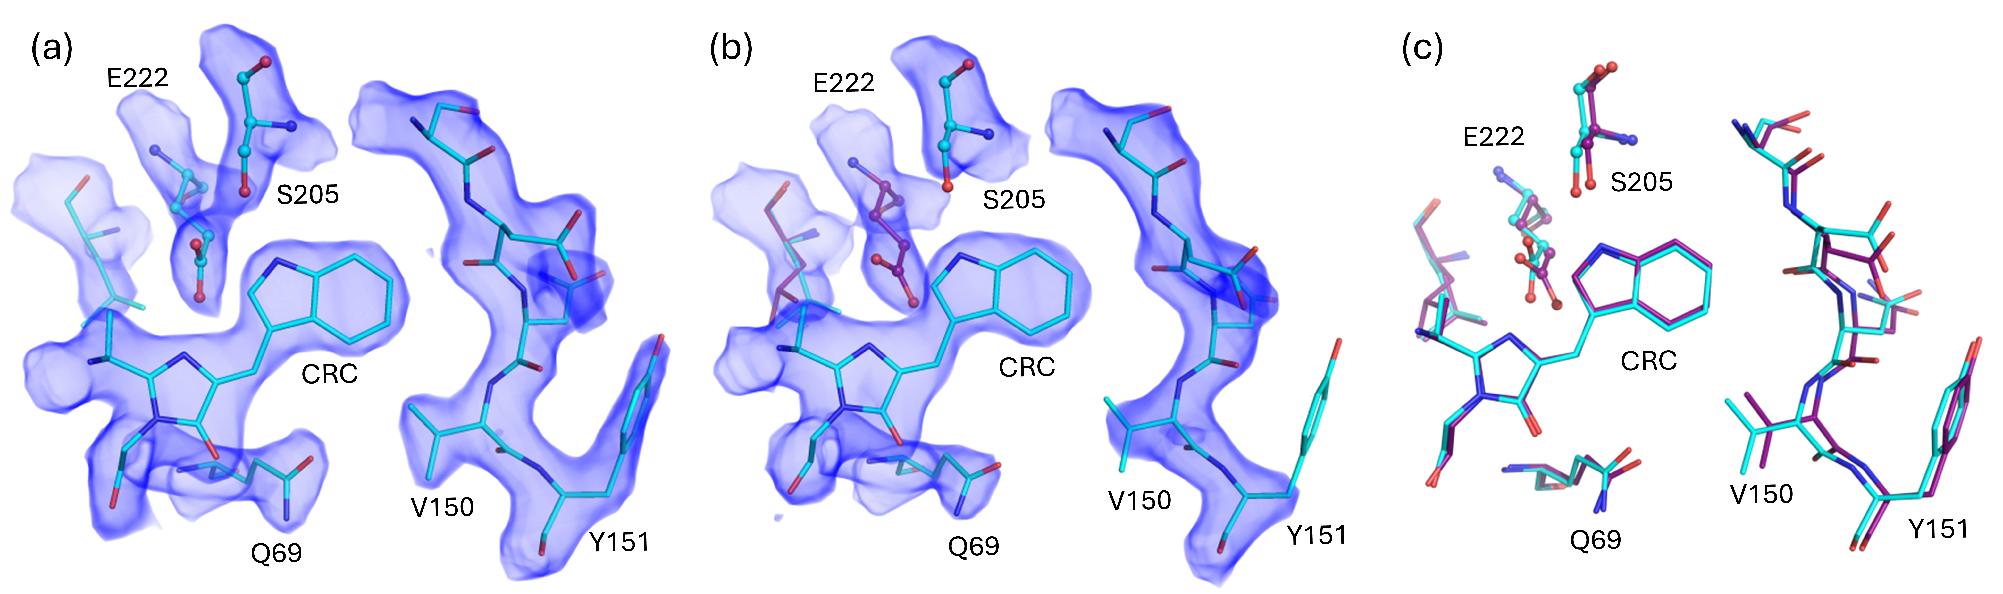
\includegraphics[width=\textwidth]{images/T-Cer/ID29_tape-drive_results.pdf}
    \caption{Results of the ID29 tape drive beamtime. 2\(F_{obs} - F_{calc}\) electron density map contoured at 1 r.m.s.d overlaid on key amino acids of the chromophore pocket. (a) In REF-TPD-ID29 (2.2 \AA\ resolution), the H-bond coordination of the chromophore is comparable to that of the cryogenic neutral pH structure, and all amino acids of the 7\textsuperscript{th} strand are well resolved. (b) 60S-TPD (2.4 \AA\ resolution) features the characteristic rotation of the carboxylic head of E222 (purple). In addition, the density on S205 is not well resolved, indicating that it has now become flexible. Both the side chains of V150 and Y151 have lost some of their electron density, indicating an increase in the flexibility of the 7\textsuperscript{th} strand. Finally, one side of N69 is no longer resolved, indicating that it has now become flexible. (c) superposition of the reference state (cyan) and 60s (purple) models, highlighting the rotation of E222 away from S205 as well as the movement of N69. The entire strand of the 7\textsuperscript{th} strand is coherently moving away from the chromophore (0.3 \AA\ distance between the C\textalpha of both V150). Finally, Leu 42 now exhibits an additional conformation (purple).}\label{fig:ID29_results}
\end{figure}

\section{Short T-Cer construct with enhanced flexibility enables \textit{in crystallo} chromophore isomerisation}

We identified two factors preventing the configuration switch of T-Cer's chromophore \textit{in crystallo} after a mixing-induced pH drop: the main one is the rigidity of the crystalline packing, which prevents a necessary movement of the 7\textsuperscript{th} strand, and the lesser one is the viscosity of the crystal suspension, which slows down diffusion. 

To further increase the flexibility of T-Cer \textit{in crystallo}, a construct where the C-terminus is removed (T-Cer-s) was designed (Section \ref{sec:short}). To decrease the viscosity of the crystal suspension, a new crystallisation condition and protocol were designed, where the precipitant is now NH\textsubscript{4})\textsubscript{2}SO\textsubscript{4}.  

To assess whether these innovations allow the switch of the chromophore of T-Cer-s from configuration Z,Z to E,Z \textit{in crystallo}, crystals were soaked in pH 4.0 sodium citrate. 

\subsection{Soaking T-Cer-s crystals obtained in ammonium sulfate}\label{sec:soaking}

\subsubsection{Soaking and cryo-trapping}

One such crystal, cryo-cooled after 150 s of soaking (150S-CT-S) features a negative \(F_{obs} - F_{calc}\) peak on the nitrogen atom of the indole ring of configuration Z,Z, and a twin positive peak corresponding to the position of the nitrogen atom of the indole ring in configuration E,Z configuration  (Fig. \ref{fig:T-Cer-soak-struc} (a)). 

In 150S-CT-S, a negative electron density peak on the carboxylic head of E222 indicates its departure from the REF-like conformation (Fig. \ref{fig:T-Cer-soak-struc} (a)). Additional negative peaks on the side chains of V150 and Y151, coupled with an array of positive peaks on the solvent side of the 7\textsuperscript{th} strand, indicate that it is partially 'translated'. A negative peak on the carbon of N69, coupled with a positive, two-sided density pattern above it, perfectly reflects the difference in conformation of N69 between the MZZ state and aged crystals (Fig. \ref{fig:T-Cer_pH8vs4} (b) and (d)). Positive peaks on the side of the imidazolinone ring  suggest that it moves up lightly, to allow to switch to configuration E,Z. Finally, a faint positive peak between V150 and N69 even hints at the existence of the new stable water molecule coordinating the chromophore when it is in the E,Z configuration, visible in Fig. \ref{fig:ageing_struc} (c).

\vspace{2mm}

\textbf{This is irrefutable proof that the switch from configuration Z,Z to configuration E,Z can occur \textit{in crystallo}, and validates the relevance of using the T-Cer-s construct and crystallising in  (NH\textsubscript{4})\textsubscript{2}SO\textsubscript{4}. }

Cryo-cooling crystal can favour specific conformations \parencite{fraserHiddenAlternateStructures2009,fraserAccessingProteinConformational2011}. The E,Z configuration has, so far, only been observed at cryogenic temperature; to validate its relevance, it was important to assess whether it could also be observed at room temperature. 

\subsubsection{Soaking, and collection at room temperature.}

A crystal was soaked for 60 s and mounted on the goniometer directly, protected by the flow of a humidity controller \parencite{sanchez-weatherbyImprovingDiffractionHumidity2009}, and collected after 180 s in total (180S-RT-S).

180S-RT-S showcases similar features as 150-CT-S, most notably a positive peak under the chromophore, indicating the existence of the E,Z configuration  ((Fig. \ref{fig:T-Cer-soak-struc} (b)). Features identified on E222, N69 and the full 7\textsuperscript{th} strand are also present and stronger than in 150-CT-S despite the lower resolution of 180S-RT-S.

\textbf{We can, at long last, validate that the E,Z configuration of the chromophore is induced by dropping the pH from 8.0 to 4.0 in a T-Cer-s crystal. }

Two questions are immediately prompted by this finding: (1) Is this E,Z configured species the same as that which is formed at acidic pH in solution? (2) If so, how fast does the configuration switch happen \textit{in crystallo}?

\subsubsection{\textit{in crystallo} configuration switch, monitored by \textit{ic}AS}

Crystals of T-Cer-s grown at neutral pH (sGS-CT) were soaked for 30 s (s30S-CT) and 120 s (s120S-CT), then cryo-cooled using the cryo-stream of the main \textit{ic}OS setup before their \textit{ic}AS spectra were recorded. 
 
The main absorption band of sGS-CT (coloured blue in Fig. \ref{fig:T-Cer-soak-struc} (a)) is blue-shifted from 440 nm to 410 nm in s30S-CT (orange) while conserving its two-peaked nature. It red-shifts back to 430 nm in s120s-CT (green), which matches the signature of T-Cer in solution at pH 4.0 (red spectrum in Fig. \ref{fig:T-Cer_insolution_pH_static}). All spectra recorded after longer soaks than s120s-CT showcased the same signature. 

\vspace{2mm}

\textbf{We can validate that the E,Z configured species created by a pH drop in a T-Cer-s crystal is very likely the same species formed in solution at acidic pH. }

\vspace{2mm}

The E,Z configured species forms within 120 s and not before 60 s in smaller (\(100 \times 20 \times 20 \) \textmu m\textsuperscript{3}) crystals of T-Cer-s. Even though it is much slower than in solution, characterising this transition could prove interesting. 
\begin{figure}[H] %bt!]
    \centering
        \noindent 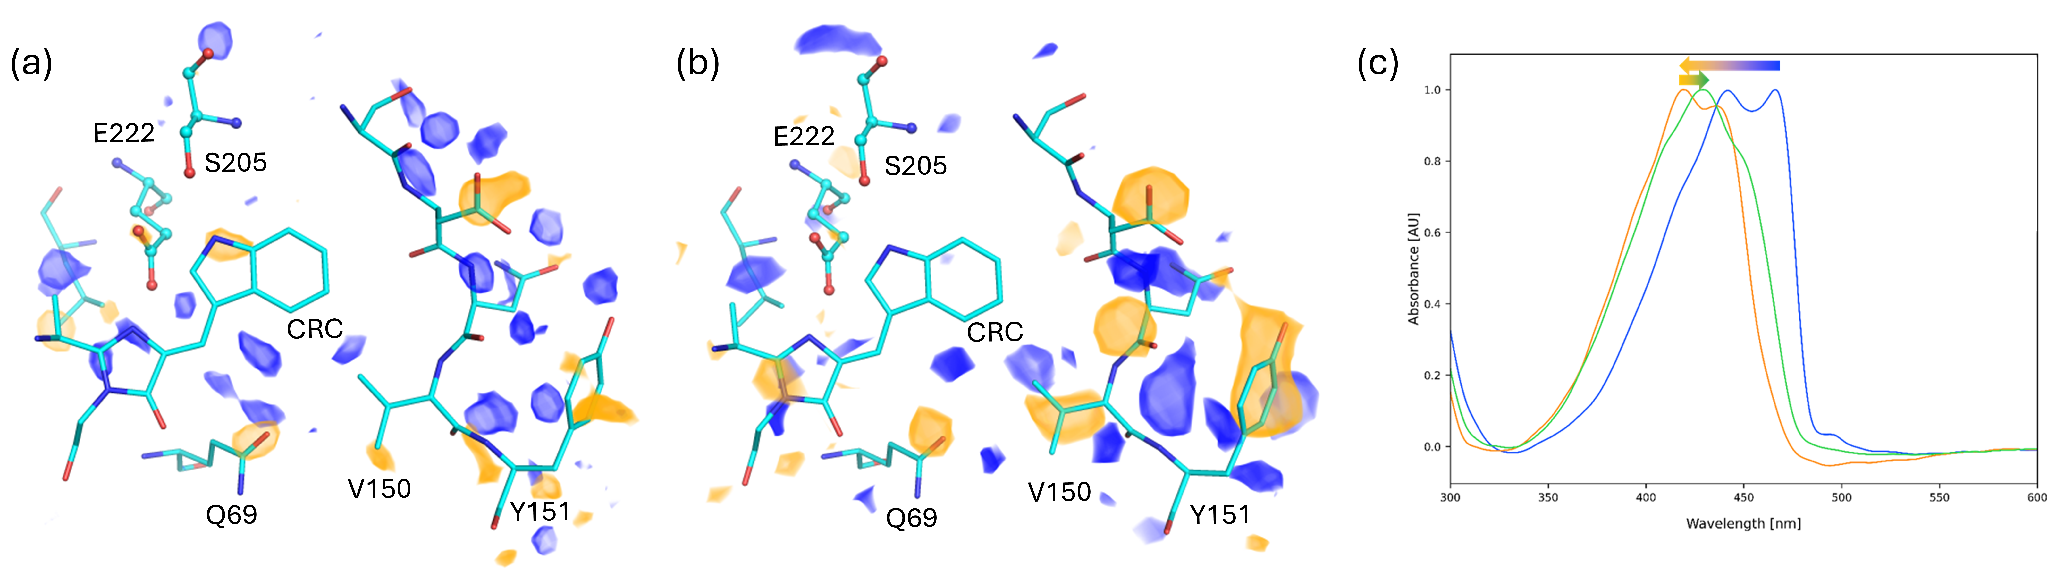
\includegraphics[width=\textwidth]{images/T-Cer/T-Cer_soaking.pdf}
    \hfill
    \caption{Soaking macro-crystals (\(\sim 200 \times 50 \times 50\) \textmu m\textsuperscript{3}) of T-Cer-s obtained in ammonium sulfate. Electron difference density map (\(F_{obs} - F_{calc}\) contoured at 3.0 r.m.s.d, positive peaks in blue, negative peaks in gold. and overlaid on the model for REF-S. (a) 150S-CT-S (1.3 \AA\ resolution), contoured at 3.0 \textsigma\ level) The negative peak on the nitrogen atom of the indole ring in the chromophore, along with a positive peak \textasciitilde 3.5 \AA\ lower, where the nitrogen atom would be in configuration E,Z,  suggests that part of the chromophore has changed from the Z,Z configuration to the E,Z configuration. Additionally, a small negative peak on E222 indicates a loss of some of the neutral pH conformation of E222. Pairs of peaks on each side of the amino acids of the 7\textsuperscript{th} strand are backing away from the chromophore. Negative peaks on the side chains of V150 and Y151 show that a fraction of them are becoming flexible. A negative peak on the head of N69 shows that it is also becoming partially flexible. 
    (b) 180-RT-S (2.2 \AA\ resolution) features a positive peak where the nitrogen atom of configuration E,Z would be. There is also a strong negative peak on V150 and Y151, as well as positive peaks on the outer side of the 7\textsuperscript{th} strand amino acids, indicating the backing-away movement and enlargement of the chromophore pocket. A positive peak on the bottom right of Y150 indicates that it has partially tilted to adopt its low pH conformation. A negative peak on N69 indicates that it has become partially flexible too. 
    (c) sGS-CT (blue), s30S-CT (orange) after s120S-CT (green) represented with coloured arrows indicating the transitions between them. sGS-CT is similar to sGS (Fig. \ref{supfig:pH8_spec}). In s30S-CT, the main absorption band of the chromophore has blue-shifted to feature a peak at 410 nm and a weaker one at 435 nm. In s120S-CT (green), the main absorbance peak has red-shifted to 430 nm, and the absorption band presents shoulders at 450 nm and 400 nm., similar to s15D (blue in Fig. \ref{fig:ageing_spec})}\label{fig:T-Cer-soak-struc}
\end{figure}

\subsection{Monitoring the rise of the E,Z configuration via TR-MX with the ALD setup}

Thanks to a collaboration with Takashi Tomizaki, beamline scientist of beamline PXI - X06SA (PXI) at the Swiss Light Source (SLS), Paul Scherrer Institute (PSI), we were offered commissioning beamtime for the TR-MX setup developed on PXI, using an Acoustic Levitation device (ALD, \cite{tsujinoUltrasonicAcousticLevitation2016, kepaAcousticLevitationRotation2022}, described further in Section \ref{sec:ALD}). Crystals of T-Cer S were collected in their reference state (REF-ALD), 150 s (150S-ALD) and 300 s (300S-ALD) after they had been mixed with acidic buffer (protocol described in section \ref{sec:ALD_protocol})

In 150S-ALD and 300S-ALD, E222 has adopted the MZZ-like conformation, which validates that the crystals have been subjected to a pH drop (Fig. \ref{fig:ALDresults} (b) and (c)). However, the entire scaffold of T-Cer-s, on the side of V150, is displaced compared to the reference state in datasets collected after mixing, while the top of the \textbeta-barrel, specifically the loop carrying P192, is displaced towards the inside of the barrel. This deformation movement has not been observed in any of the previous experiments. In both 150S-ALD and 300S-ALD, however, the chromophore remained entirely in the Z,Z configuration. 

Additionally, dehydration of the sample could be observed for the 150 s and 300 s time point datasets: the drop containing the crystals shrunk over time. This phenomenon was so pronounced that the height of the nanodisk had to be adjusted (lowered) to collect the 300 s dataset. 

\vspace{2mm} 

Therefore, while this experimental scheme succeeded in inducing a pH drop in T-Cer-s crystals, the lack of humidity control made it unfit for probing long delays after mixing. The crystals of T-Cer dehydrated, which has been shown to prevent isomerisation (Section \ref{sec:soaking_protocol}).  
\begin{figure}[H] 
    \centering
        \noindent 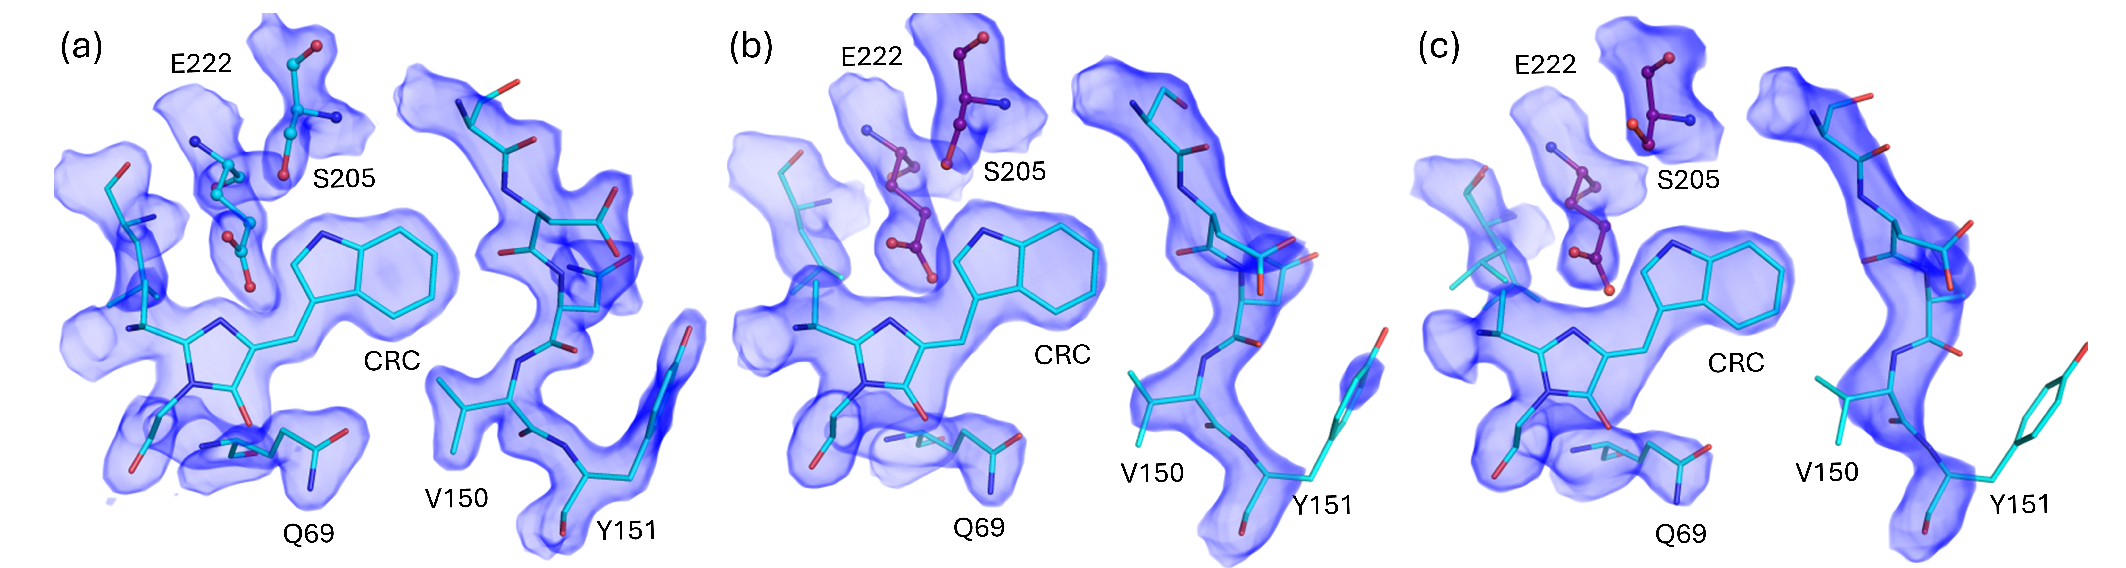
\includegraphics[width=\textwidth]{images/T-Cer/ALDresults.pdf}
    \caption{Structures of datasets collected with the ALD setup. 2\(F_{obs} - F_{calc}\) electron density maps of T-Cer-s crystals at neutral pH, reference state, contoured at 1.0 r.m.s.d (a) REF-ALD (2.2 \AA\  resolution). (b) 150S-ALD, (2.5 \AA\  resolution), showing the movement of the 7\textsuperscript{th} strand away from the chromophore, as well as the rotation of E222 and flexibility of Y151 (c) In 300S-ALD, (2.7 \AA\  resolution), Y151 appear to be completely dynamic, while S205 is completely disengaged with the chromophore.}\label{fig:ALDresults}
\end{figure}

\subsection{Discussion}

Crystals of T-Cer-s grown in  (NH\textsubscript{4})\textsubscript{2}SO\textsubscript{4} based crystallisation conditions displayed enhanced flexibility \textit{in crystallo} and tolerated soaking experiments better than T-Cer crystals grown in PEG, up to the point that the switch from configuration Z,Z to configuration Z,Z could finally happen \textit{in crystallo} in seconds, and not days. However, despite these improvements, the configuration switch remained much slower than in solution and crucially too slow to be studied by TR-MX. 

V150 holds a pivotal role in controlling the configuration of the chromophore of T-Cer. \textit{In crystallo}, it de-correlates the isomerization of the chromophore from the pH, by adding in a 'lag period' corresponding to the large-scale rearrangement of the 7\textsuperscript{th} strand, which must be completed to move V150 out of the way of the E,Z configuration. The mutation T65A on Cerulean created a fast-switching variant in solution. Mutating V150 to a less bulky amino acid could remove the dependency of the isomerization on the movements of  the 7\textsuperscript{th} strand and create a fast isomerising variant \textit{in crystallo}.

\section{Elucidating the gating effect of V150 on the isomerization of T-Cer's chromophore} \label{sec:V150A}
\subsection{High-resolution structures of the new variant V150A at neutral and acidic pH}
Ready-to-freeze crystals (protocol described in Section \ref{sec:highrescryst}) of a construct of T-Cer-s where V150 is replaced by a less bulky alanine, V150A (described in section \ref{sec:V150A}) were grown at pH 8.0 (8-V150A) and 4.0 (4-V150A), fished and cryo-cooled using the cryo-stream of the beamline.  

The chromophore of 8-V150A is mainly (80 \%) adopting the same configuration as in REF, with H-bonded S205 and E222 (cyan in Fig. \ref{fig:V150Astructure} (a)). However, a small population (20 \%) adopts an 'untethered' conformation while still being in the Z,Z configuration (not unlike MZZ), where the chromophore is no longer H-bonded to S205, and is now angled down, slightly more towards A150 (green in Fig. \ref{fig:V150Astructure} (a)). Interestingly, though, the conformation of E222 is not significantly affected by the existence of the untethered chromophore. 

Strikingly, the chromophore in 4-V150A adopts the Z,E configuration (purple in Fig. \ref{fig:V150Astructure} (c)) observed in crystals of Cerulean obtained at slightly acidic pH (5.0) (Fig. \ref{fig:Cerulean_pH} (a), \parencite{gotthardChromophoreIsomerStabilization2017a}. A lower occupancy 'untethered' Z,Z configuration remains (cyan in Fig. \ref{fig:V150Astructure} (c)). The entire chromophore pocket of 8-V150A is involved in a network of alternate conformation coordinating the Z,E (purple in Fig. \ref{fig:V150Astructure} (c)) and Z,Z (grey in Fig. \ref{fig:V150Astructure} (c)) configurations of the chromophore. The change of conformation of the amino acids in the chromophore pocket to accommodate the Z,E configuration is massive, most notably, D148 flips inside the chromophore pocket from the outside of the \textbeta-barrel (purple vs grey conformations of D148 in Fig. \ref{fig:V150Astructure} (c)).

V150A was intended to be a 'fast switching' variant \textit{in crystallo}. Therefore, we needed to assess whether the chromophore would switch configuration after a pH drop, and if so, whether it would switch to the E,Z or Z,E configuration. Finally, we needed to ascertain whether V150A was indeed a fast-switching variant, regardless of the configuration to which it switched. 

\subsection{Soaking crystals of V150A}

A crystal of V150A grown at pH 8.0 was soaked for 10 s in pH 4.0 buffer (10S-V150A) before being cryo-cooled (detailed procedure in \ref{sec:soaking_protocol}). Longer soaks were not tolerated by the crystals. 

The chromophore of 10S-V150A has fully adopted the 'untethered' Z,Z configuration, which was marginally present in 8-V150A (green in Fig. \ref{fig:V150Astructure} (b)). S205 is almost entirely disengaged in 10S-V150A (purple conformation, 80\% occupancy in Fig. \ref{fig:V150Astructure} (b)), which at the very least supports a 60 \% conversion from the 'neutral pH' Z,Z configuration to the untethered Z,Z configuration. Finally, E222 is also fully disengaged from S205 and is particularly dynamic (Adopting an array of conformation between the green and purple conformation modelled in Fig. \ref{fig:V150Astructure} (b)), which supports it being in the protonated, glutamic acid, state. The rest of the chromophore pocket (grey in Fig. \ref{fig:V150Astructure} (b)) is unaffected. 

\vspace{2mm}

A short soak in pH 4.0 buffer produced a large difference between 8-V150A and 10S-V150, suggesting that V150A crystals are more susceptible to pH drops. However, despite E222 being protonated, the chromophore remains in the configuration Z,Z in 10S-V150A. In fact, V150A does not appear to switch configuration upon pH drop, at least before the crystals fall apart. \textbf{Therefore, V150A is not a fast-switching variant in crystallo. }
\begin{figure}[H] 
    \centering
        \noindent 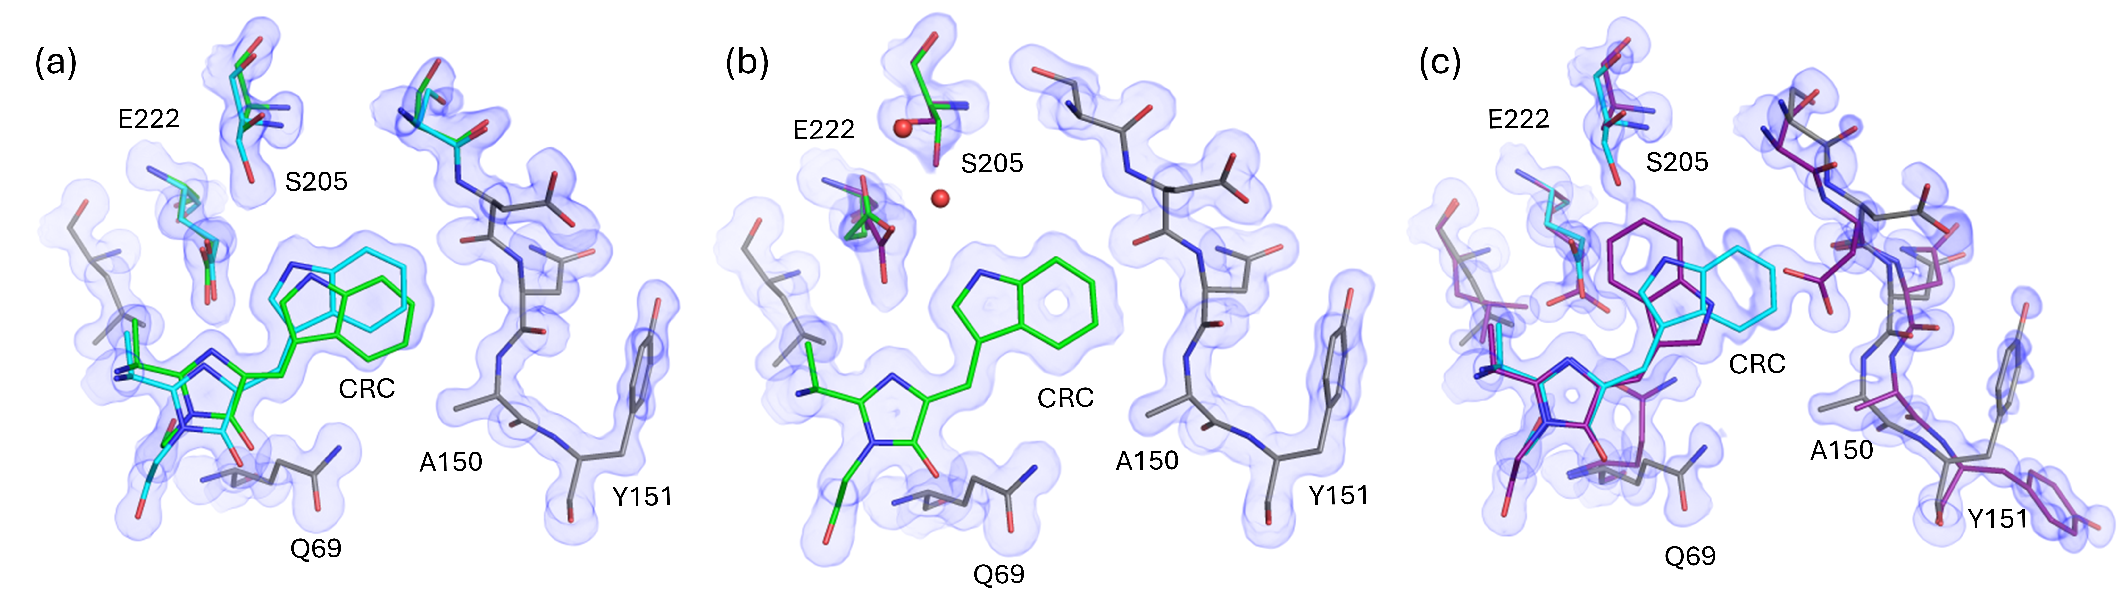
\includegraphics[width=\textwidth]{images/T-Cer/V150A_2.pdf}
    \caption{Atomic models of  V150A at different pH, with corresponding 2\(F_{obs} - F_{calc}\) electron density map overlaid on key amino acids of the active site, contoured at 1 \textsigma\ level (a)  8-V150A (1.1 \AA\ resolution) showing a network of alternate conformations of the chromophore,  S205 and E222. (b) 10S-V150A showing a unique conformation of the chromophore, and a network of alternate conformations encompassing S205 and E222, where the position of the hydroxymethyl group of S205 is replaced by a stable water molecule once it is no longer H-bonded to the chromophore. (c) 4-V150A (1.0 \AA\ resolution), showing the chromophore in alternate configuration Z,Z or Z,E. Coordinated with the two configurations of the chromophore, a network of alternate conformations comprises almost all amino acids in the chromophore pocket.}\label{fig:V150Astructure}
\end{figure}
\subsection{Discussion}

Removing the bulky side-chain of V150 did not produce the expected  \textit{in crystallo} fast-switching variant. Contrary to the original intention, it seems removing some of the bulk of the side chain of V150 has not restored the correlation between the configuration of the chromophore and pH \textit{in crystallo}, but further decreased it by de-correlating the configuration of the chromophore from the protonation state of E222, as evidenced by the existence of the 'untethered' conformation of the chromophore in 8-V150A, which remains in the Z,Z configuration without the need for stabilisation via the H-bond network involving S205 and E222. 

\vspace{2mm}

Because the chromophore's imidazolinone ring no longer moves with E222 as it gets protonated and because more space is made available to it, it ceases to switch to the more volume-conserving E,Z configuration and chooses the Z,E configuration instead. This proves that the breathing motions of the 7\textsuperscript{th} strand govern the pathway of the configuration switch. 

\vspace{2mm}

Finally, the lattice parameters of 8-V150A, 4-V150A and 10S-V150A are virtually identical (Table \ref{tab:structure-list}), which proves that there is some degree of correlation between the transition from configuration Z,Z to E,Z and the lattice parameter shrinkage over pH observed for T-Cer and T-Cer-s (Table \ref{tab:structure-list}).

\vspace{2mm}

Therefore, two novel insights can be produced from the study of the V150A variant:
\begin{itemize}
    \item The pH sensing capability of T-Cer is intrinsically tied to the presence of a bulky amino acid, pushing its chromophore against S205 and E222. 
    \item The configuration adopted by the chromophore at acidic pH is governed by directions of freedom made available by the 7\textsuperscript{th} strand of the \textbeta-barrel. 
\end{itemize}



\section{Methods}\label{sec:T-Cer_methods}

\subsection{Transformation, Expression and Purification of T-Cer}
Vectors bearing the T-Cer construct were transformed into the Escherichia coli host strain BL21 (Invitrogen) and grown on ampicillin (100 mg/ml) selective agar plates. Cells were grown in ZYP-5052 medium supplemented with ampicillin (100 mg/ml) at 37°C until an optical density of 1.2 at 600 nm was reached. ZYP-5052 (10g tryptone, 5g yeast extract, 25 mM (NH\textsubscript{4})\textsubscript{2}SO\textsubscript{4}, 50 mM KH\textsubscript{2}PO\textsubscript{4}, 50 mM Na\textsubscript{2}PO\textsubscript{4}, 0.05 D-glucose, 0.5 \% Glycerol and 0.2 \% A-lactose, pH adjusted to 7.0) was used instead of standard LB medium because Sylvain Aumonier obtained better yields with it during his PhD \parencite{aumonierTimeresolvedMonochromaticSynchrotron2019}. Protein expression was then induced with 0.1 mM IPTG and cells were grown overnight at 37°C. Cells were harvested and centrifuged at 4000 g for 20 min at 4 \degree C. Pellets were resuspended in 25 ml of lysis buffer [50 mM Tris pH 8.0, 300 mM NaCl, 0.25 mg/ml lysozyme, 400 mg/ml DNAse I, 20 mM MgSO\textsubscript{4}, 1 tablet of the EDTA-free protease inhibitor cocktail cOmplete (Roche, Basel, Switzerland)] per litre of centrifuged medium and frozen at -80°C. Thawed pellets were sonicated at 40\% intensity following a 20s on / 40s off pattern, then cell debris were centrifuged at 15 000 g, for 45 min at 4 \degree C. The protein was purified from the clarified lysate using a nickel affinity column (His-Trap HP 5 ml, GE HealthCare) and cleaned with a first step at 10 mM imidazole and a second at 20 mM imidazole then eluted against an imidazole gradient (50 mM Tris pH 8.0, 300 mM NaCl, 20–1000 mM imidazole over 70 ml). Collected fractions were then dialyzed against 100 mM Tris pH 8.0 and 300 mM NaCl buffer to remove imidazole. A second purification step consisted of size-exclusion chromatography (HiLoad 16/600 Superdex 75 pg, GL, GE HealthCare) in a 50 mM Tris pH 8.0 buffer, after which the purified protein was concentrated to 20 mg/ml.

\subsection{Crystallisation of T-Cer}\label{sec:mat_cryst}
T-Cer macro-crystals grow overnight using the hanging-drop vapour diffusion technique. Close to physiological pH (7-8), the condition us buffered using HEPES, with 50 mM MgCl\textsubscript{2} and using PEG 4000 (Sigma, BioUltra) as a precipitant, with concentrations varying from 10 to 20 \%. These conditions are detailed in \cite{lelimousinIntrinsicDynamicsECFP2009,aumonierTimeresolvedMonochromaticSynchrotron2019}. To crystallise T-Cer at a lower pH, HEPES was substituted for MES (pH 6.5,6.0) and then sodium citrate (pH 5.5-4.0).  T-Cer crystallises in space group P2\textsubscript{1}2\textsubscript{1}2\textsubscript{1}, with a solvent content of 42 \%, its lattice parameters are displayed in Table \ref{tab:structure-list}.

\subsubsection{From macro-crystals to microcrystals} \label{sec:microcrystallisation}
Obtaining a size homogeneous micro-crystalline slurry with the ‘traditional’ vapour diffusion methods is challenging, because the trajectory of the medium in the drop through the phase diagram is not easy to ascertain, and therefore the time spent in the metastable (growth) zone cannot be estimated accurately for each drop \parencite{bealeSuccessfulSamplePreparation2019}. Furthermore, there are ‘edge effects’ at the interface of evaporation, creating inhomogeneously sized crystals. As a consequence, a condition producing the desired size of crystal in a drop of 1-2 \textmu l might no longer produce the desired crystals once the volume is scaled up. Finally, scaling up crystal production past a certain point with hanging drop vapour diffusion is impossible, as the crystalline slurry will need to be harvested and pooled into a larger container, and a significant portion of the sample will be lost during that step. 

This is why most SX experiments are performed with crystals grown in batches. In its simplest form, batch crystallisation relies on hitting the nucleation zone right as the protein is mixed with the precipitants \parencite{mcphersonPreparationAnalysisProtein1982}. Because there is no evaporation and subsequent concentration of the crystallisation solutions, the only variable to change in a protein batch over time is the protein concentration in the solution, decreasing as crystallisation happens. This makes for a much simpler trajectory in the phase diagram (see Fig. \ref{fig:Crystallisation_T-Cer} (a)).
Hitting the nucleation zone right as the different components of a batch crystallisation condition are mixed is challenging. Controlling crystal size with this method means being able to ensure the correct number or nucleation point (which is governed by the time spent in the nucleation zone) and the correct amount of crystal growth (which is governed by the combined times spent in the nucleation zone and meta-stable zone). This is impossible for most systems. Fortunately, the nucleation step can be 'bypassed' by using crystal seeds: extremely small crystalline particles which will act as a platform for crystal growth or facilitate nucleation \parencite{mcphersonPreparationAnalysisProtein1982,bergforsSeedsCrystals2003}. With this method, controlling the number of crystals becomes as simple as controlling the number of seeds added to the medium (provided 'natural' nucleation does not happen). Further, the batch condition can be aimed directly at the (usually much larger) meta-stable zone (Fig. \ref{fig:Crystallisation_T-Cer} (b) represents examples of a trajectory attainable with seeded batch crystallisation). This means that the only variable to adjust to get correctly sized crystals is the time spent in the meta-stable zone, which is much more manageable. 
\begin{figure}[H] %bt!]
    \centering
        \noindent \includegraphics[width=\textwidth]{images/T-Cer/Crystallisation_T-Cer.pdf}
    \hfill
    \caption{Engineering microcrystals of T-Cer. (a) Schematic phase diagram of a batch crystallisation experiment. The nucleation zone is coloured in green, the meta-stable zone is coloured in blue and the precipitation zone is coloured in red. The red dotted arrow represents possible linear, downward trajectories taken by crystallisation batches as the concentration of protein in solution decreases with crystallisation. (b)  Schematic phase diagram of a seeded batch crystallisation experiment. The colour codes are unchanged from (a). The use of seeds allows to exploitation of a much larger zone of the phase diagram because hitting the nucleation zone is no longer needed since crystal growth can occur around seeds, as evidenced by trajectories V, VI and VII. Both (a) and (b) are reproduced from \cite{bealeSuccessfulSamplePreparation2019} (c) 10 \textmu l micro-batches of T-Cer set-up with identical crystallisation conditions (100 mM HEPES at pH 8.0;  20 \% PEG; 50 mM MgCl\textsubscript{2}; 1:3 protein), but seeded with increasing concentration of crystal seeds. If no seeds are added to the mix, only phase transition is visible in the batch. If 1 \textmu l of a 1/1000 diluted seed stock is added to the mix, \textasciitilde 50 large (\(100 \times 100 \times 50\) \textmu m\textsuperscript{3}) crystals grow. If 1 \textmu l of a 1/10 diluted seed stock is added to the mix, a slurry of micro-crystals grows.  (d) Crystals grown in the final conditions scaled for a batch volume of 1.5 ml (100 mM HEPES at pH 8.0;  25 \% PEG; 50 mM MgCl\textsubscript{2}; 1:3 protein), with a constant thickness of \textasciitilde 5 \textmu m. (e) Sample tube sent to PETRA III in prevision of the beamtime, with clear sedimentation of the crystal pellet.}
    \label{fig:Crystallisation_T-Cer}
\end{figure}
Crystal seeds of T-Cer were first prepared by crushing large (\textasciitilde 500 \textmu m) crystals fished from 12 hanging drop wells using a tissue grinder (protocol described in \parencite{aumonierTimeresolvedMonochromaticSynchrotron2019}). The large crystals were re-suspended in a solution with the same composition as their mother liquor and reference for 5 minutes. The resulting slurry was stored in an Eppendorf tube and characterised under a microscope. This approach is quick and straightforward, but large (> 10 \textmu m) particles remain in the solution, amid smaller barely visible seeds. This introduces inhomogeneity in the size distribution of crystals grown with seeded batches. To solve the size inhomogeneity issue, the large crystals harvested were crushed with ceramic seeding beads (Hampton research, HR4-781 - Seed Bead Ceramic Kit) instead of a tissue grinder. 6 seeding beads were added to an Eppendorf tube containing large crystals harvested and re-suspended in 200 \textmu l, before it was shaken for 25 minutes using a vortex 'hands-off' attachment, at medium speed to minimise friction-induced heat. The resulting seed suspension was observed under a microscope to validate that it contains only \textasciitilde  \textmu m or smaller particles.

Microbatches are medium-sized (10 \textmu l) droplets set in sitting drop plates, covered in oil to prevent evaporation (See \cite{chayenMicrobatchCrystallizationOil1992} for a precise description of the method). They were used to bridge the gap between known hanging drop vapour diffusion conditions yielding microcrystals of T-Cer and the desired batch condition.  Microcrystals of T-Cer can reliably be obtained via the hanging-drop vapour diffusion method with the following conditions: 30\% PEG 4000, 100 mM HEPES pH 8.0, 50mM MgCl2, 1/1 ratio of 20 mg/ml T-Cer. Arrays of micro-batch trials were started around this condition screening for protein concentration (by adjusting the protein/mother-liquor ratio of the mix) and precipitant concentration. The micro-batches were set in sitting drop plates to allow daily observation with a microscope.  It is possible to identify conditions where the concentration of T-Cer seeds governs crystal growth, as evidenced by the absence of crystal growth if no seeds are supplemented (first panel of Fig. \ref{fig:Crystallisation_T-Cer} (c)), and the strong variation in crystal size depending on the concentration of T-Cer seeds provided (visible in the second vs the last panel of Fig. \ref{fig:Crystallisation_T-Cer} (c)). If the desired state has been reached, the crystallisation can be 'quenched' by centrifuging the crystals at a moderate (3000 G) speed and resuspending them in a mother liquor of identical composition, without T-Cer.  Finally, the sedimentation of thin sand-like particles is a telltale sign of a successful batch crystallisation (Fig. \ref{fig:Crystallisation_T-Cer} (e)). 

These trials allowed to converge on an optimal condition of 20\% PEG 4000, 100 mM HEPES pH 8.0, 50 mM MgCl2, 1/1000 final dilution of the seed stock and 13.3 mg/ml final concentration of T-Cer for crystal growth.  This condition yielded crystals of a homogeneous thickness (5 \textmu m, Fig. \ref{fig:Crystallisation_T-Cer} (d)). Several sample tubes (Fig. \ref{fig:Crystallisation_T-Cer} (e)) were sent to PETRA III to plan the beamtime. Crystals were also grown on-site with the help of the P11 beamline staff, using seeds made from one of the sent batches, showcasing the robustness of this protocol. 

\subsubsection{Growing high-resolution diffracting crystals}\label{sec:highrescryst}

The size of the crystal was increased to further enhance the diffracting resolution. This was achieved by using a PEG concentration of 10 \%, too low to allow nucleation of the protein on its own (See Fig. \ref{fig:Crystallisation_T-Cer} (c)), and further decreasing the concentration of crystal seeds supplemented to 1/100 000. Protein concentration was maintained at 20 mg/ml. As a result, the sample which would have been used for the growth of many \textasciitilde 20-50 crystals was funnelled into the growth of 1 - 3 larger (\(\sim 200 \times 100 \times 100 \) \textmu m\textsuperscript{3}) crystals. Transferring a crystal into a drop of cryo-protectant causes mechanical stress, for instance, T-Cer and its variants' crystals melt when they are soaked in glycerol. As a final step, we used the crystallisation condition outlined above, supplemented with 20 \% V/V glycerol, and produced large, cryoprotected T-Cer crystals.

\subsubsection{Ammonium sulfate crystallisation condition to improve mixing}\label{sec:ammonium}

PEG, as a viscous agent, has been shown to inhibit the transfer of protons from the bulk solvent to the chromophore pocket of the GFP \parencite{saxenaProteinDynamicsControl2005}. This is due to PEG inhibiting protein dynamics and preventing the normal function of proton shuttling pathways. PEG also slows down the diffusion rate of small molecules in crystals and their mother liquor (\cite{makinenReactivityCryoenzymologyEnzymes1977}, Tomizaki Takashi (PSI), Sylvain Engilberge (IBS), personal communication \footnote{In particular, the diffusion rate of several coloured dyes in protein crystals and their mother liquor was assed with the acoustic levitation device currently being commissioned on PXI \parencite{tsujinoUltrasonicAcousticLevitation2016,kepaAcousticLevitationRotation2022}. Picoliter liquid dispensers were used to project droplets of dies on droplets containing protein crystals. The mixing time was assessed using a high-speed camera. Mixing times were noticeably higher (tens of seconds for PEG-based crystallisation conditions vs 100s of ms for salt-based conditions).}). PEG is also known to block substrate diffusion channels \parencite{barrettInsightsRedoxPartner2004}. T-Cer crystals are obtained in very high molecular weight (4000) PEG. These long molecules induce molecular crowding, which could also participate in slowing down the movements of the \textbeta-sheets in T-Cer and T-Cer-s crystals. 

Fluorescent proteins have been crystallised in salt-based conditions before. A survey of the Protein Data Base, as well as a personal communication from Nicolas Coquelle, directed me to the crystallisation condition of rsEGFP2 at neutral pH used for the TR-SFX measurements of \cite{coquelleChromophoreTwistingExcited2018}. However, T-Cer-s is significantly different from rsEGFP2. As a consequence, T-Cer transitioned from soluble to semi-amorphous particles (Fig. \ref{fig:T-Cer-NH4} (a)) without ever crystallising. Screening around the condition did not yield any crystalline particles. 

Based on the personal experience that rounds of seeding would improve the quality of crystals and microcrystals, a seeded crystallisation trial was prepared in a condition containing both PEG 4000 and ammonium sulfate, with seeds prepared from crystals grown in PEG-based conditions with the P 2\textsubscript{1} 2\textsubscript{1} 2\textsubscript{1} crystal packing. This trial proved that crystals could be grown if the crystallisation drop was seeded in a condition containing 15\% PEG and 0.5 M ammonium sulfate (Fig. \ref{fig:T-Cer-NH4} (b)). The crystals grown in these conditions were harvested to make a new preparation of crystal seeds (see Section \ref{sec:microcrystallisation} for the protocol). The process was repeated several times, with increments of 5 \% diminution of the concentration in PEG, and 0.25 M augmentation of the concentration in ammonium sulfate, and using the previous trial as a base for the preparation of seeds. The final condition contained only 100 mM of Hepes and 2 M ammonium sulfate and yielded satisfyingly sized homogeneous micro-crystals (Fig. \ref{fig:T-Cer-NH4} (c)). The size of the micro-crystals can be adjusted by varying the concentration of crystal seeds. 
\begin{figure}[H] %bt!]
    \centering
        \noindent \includegraphics[width=\textwidth]{images/T-Cer/NH4_crystallisation_T-Cer-s.pdf}
    \hfill
    \caption{Engineering a crystallisation condition for T-Cer-s in ammonium sulfate. (a) Hanging drop vapour diffusion crystallisation trial of T-Cer-s. The mother liquor contains 100 mM HEPES pH 7.0 and 2 M ammonium sulfate. Only extremely small amorphous particles formed. The yellow colour of the particles indicates that T-Cer-s is not denatured. (b) Cross-seeded mixed precipitant crystallisation condition: the mother liquor contains 100 mM HEPES pH 7.0, 1M ammonium sulfate and 10 \% PEG 4000. It is seeded with T-Cer-s crystal seeds diluted 1/1000. Rectangular prism-shaped crystals (of size \(20 \times 20 \times 50 \) \textmu m\textsuperscript{3}) grew in 3 days, with a very homogeneous distribution of size.  (c) Ammonium sulfate only crystallisation condition: the mother liquor contains 100 mM HEPES pH 7.0 and 2 M ammonium sulfate. It is seeded with a preparation made from crystals grown in a mixed precipitant condition. Bi-pyramid-shaped microcrystals (of size \(20 \times 20 \times 20 \) \textmu m\textsuperscript{3}) grew in 3 days, with a very homogeneous distribution of size.}\label{fig:T-Cer-NH4}
\end{figure}
This crystallisation condition was ported to batch crystallisation with a 1:2 ratio of protein to mother liquor, a conserved final ammonium sulfate and pH buffer concentration, and a concentration of seeds divided by 3. 


\subsection{Limited proteolysis of T-Cer enhances its flexibility \textit{in crystallo}}\label{sec:limited_proteolysis}
The plasmid of T-Cer does not contain a cleavage site between the HIS-tag used for the affinity purification step and the rest of the protein, it is therefore not possible to remove it during the purification. Further, this HIS-tag is located at the C-terminus. As previously discussed (see Section \ref{sec:ageing}), the C-terminus of T-Cer adopts a different position depending on the pH. For crystals obtained at neutral pH (that is to say, all T-Cer crystals used for TR-MX experiments over the course of this project), the C-terminus is positioned away from the main \textbeta barrel of T-Cer, angled at 90 \degree. This tail is composed of semi-flexible (only the main chain is visible in the electron density map) and rigid (fully ordered, all of the amino acids are visible in the electron density) amino acids.  Upon examining the crystal packing of T-Cer at neutral pH, it appears that the C-terminal tail is stuck between neighbouring symmetry mates (Fig. \ref{fig:limited_proteolysis} (a)).  In particular, Y237 near the end of the C-terminus, is perfectly ordered and creates a crystal-contact point with the backbone of K45 from a symmetry mate. While not visible, the bulky HIS-tag is still present in the crystals and constitutes an additional source of crowding in that region of the unit cell.  

The appearance of the E,Z configuration of the chromophore after a pH drop likely requires the same movement of the 7\textsuperscript{th} strand as observed during the ageing phenomenon (Section \ref{sec:ageing}). This movement is hindered \textit{in crystallo}, which is likely in part a consequence of the rigidity of the C-terminus (Fig. \ref{fig:T_Cer_cter}). Therefore, removing the C-terminal tail of T-Cer from the protein before crystallisation might increase the flexibility of T-Cer in its crystalline form. 

Limited proteolysis has been utilised by the group of Antoine Royant (and its former members) to trim flexible parts of a protein and facilitate its crystallisation \parencite{aumonierTimeresolvedMonochromaticSynchrotron2019,gotthardCapturingBluelightActivated2023}.  In his thesis, Sylvain Aumonier describes the incubation of T-Cer with trypsin as a way to control the nucleation rate of the protein and improve his micro-crystallisation trials. The most 'accessible' part of T-Cer is its C-terminus; it is therefore likely that the main consequence of the limited trypsination of T-Cer was the removal of the tail. 

At the end of the purification, right before crystallisation, T-Cer was incubated with increasing concentration of Trypsin (5 \textmu g/ml to 5 mg/ml), and without Trypsin at 37 \degree C for 1h \footnote{This is a reproduction of the protocol detailed in Section 2.1.3 of \cite{aumonierTimeresolvedMonochromaticSynchrotron2019}. T-Cer is extremely thermostable (unfolding temperature of 84.8\degree C, unpublished data).}.  Running the incubated sample on an SDS-PAGE migration gel revealed the appearance of an additional, slightly lower molecular weight band (lanes 3:6 of Fig. \ref{fig:limited_proteolysis}) (b)) than the non-incubated proteins (lanes 1 and 8 of Fig. \ref{fig:limited_proteolysis}) (b)). This suggests that trypsin has indeed cleaved part of the protein, reproducing results of \cite{aumonierTimeresolvedMonochromaticSynchrotron2019}. 

Importantly, Trypsin self proteolyses extremely quickly. As an example, Trypsin incubated at 37 \degree C for 1h appeared as extremely low molecular weight fragments in SDS-PAGE migration. In order to obtain a band on the gel, Tryspin had to be loaded directly from the extemporaneously thawed stock, kept at 4\degree C  (lane 7 in Fig. \ref{fig:limited_proteolysis} (b)). It is therefore safe to assume that Trypsin has fully self-propolysed before the crystallisation batch is set. 
\begin{figure}[H] %bt!]
    \centering
        \noindent \includegraphics[width=\textwidth]{images/T-Cer/Limited_proteolysis.pdf}
    \hfill
    \caption{Limited proteolysis to remove the C-terminal tail of T-Cer. (a) Structure of symmetry-related molecules in a neutral-pH crystal of T-Cer. The electron density (2\(F_{obs} - F_{calc}\), 1.11 \AA\  resolution) map is represented on its C-terminal tail contoured at 1 \textsigma\ level Three of its symmetry mates (grey, pale-cyan and white) are also represented. The C-terminal tail of T-Cer at neutral pH is trapped between three symmetry mates, rigidifying it. Tyrosine 237 establishes an H-bond with the carbonyl of Lys 45 from the grey monomer, further stabilising it. This interaction is  a crystal packing point. (b) SDS-Page migration of purified T-Cer. Lanes contain (from left to right):\\
    1. T-Cer incubated at 37 \degree C without Trypsin\\
    2. Molecular weight ladder\\
    3. T-Cer and 1/10 diluted Trypsin stock\\
    4. T-Cer and 1/50 diluted Trypsin stock\\
    5. T-Cer and 1/100 diluted Trypsin stock\\
    6. T-Cer and 1/1000 diluted Trypsin stock\\
    7. Trypsin from the stock (non-incubated)\\
    8.T-Cer incubated at 37 \degree C without Trypsin\\
    9. Molecular weight ladder\\
    The red bar shows the migration front from both full-length T-Cer lanes. All conditions of T-Cer incubated with Trypsin (lanes 3:6) showcase a band of slightly lower molecular weight than non-incubated T-Cer, presumably cleaved T-Cer. Lanes  4,5 and 6 show an increasingly weaker band of the same molecular weight as non-cleaved T-Cer. The lower molecular weight band grows with Trypsin concentration, and the T-Cer molecular weight band decreases with Trypsin concentration.}\label{fig:limited_proteolysis}
\end{figure}
In preparation for the Hamburg trip, large crystals of T-cer cleaved with the protocol described above, obtained at neutral pH, were soaked in 1 M pH 4.0 Sodium Citrate buffer and cryo-cooled after a minute. They exhibited shrunken lattice parameters, which was an improvement from the results of previous soaking experiments (described at the end of Section \ref{sec:ageing}). This suggested that using pure pH buffer for the pH drop and limited proteolysis for sample preparation were indeed improvements to the protocol.

In addition to the micro-crystalline sample of T-Cer sent to Hamburg from Grenoble, T-Cer was also expressed, proteolysed and crystallised onsite directly to ensure sample quality. 

\subsubsection{Effect of the proteolysis on the lattice parameter distribution}
The C-axis of the unit cell in REF-LAMA and REF-P11-2 (crystallised with proteolysed T-Cer) is 72.6 \AA\ long (Table \ref{tab:structure-list}), a 2 \AA\ increase compared to that of REF-TPD-1 (crystallised with full-length T-Cer, Table \ref{tab:structure-list}), which supports the idea that the limited proteolysis step affects the protein packing. Otherwise, REF-LAMA is identical to REF-TPD-1 and REF, which validates that the proteolysis step does not affect the chromophore pocket. 

3 s after proteolysed crystals are shot with a droplet of sodium acetate, distinct populations (70 \AA\ long C-axis and 66.8 \AA\ long C-axis) are observed in the distribution of lattice parameters (Table \ref{tab:structure-list}). 3S-LAMA corresponds to the most abundant, short-axis population. 

The same phenomenon occurs 3 s and 8 s after proteolysed crystals are mixed with sodium acetate (Table \ref{tab:structure-list}).  Interestingly, the mix of population is only observed 3 s after mixing with sodium citrate, and the 8 s population distribution is homogeneous (short axis). 3S-TPD-Ac, 3S-TPD-Ci and 8S-TPD-Ac correspond to the 66.8 \AA\ population.

The existence of several species in the distribution of lattice parameters during serial data processing with CrystFEL is puzzling. This may be a consequence of an inhomogeneous cleavage of the C-terminus by the limited proteolysis step, leading T-Cer to form crystals made of monomers all cleaved in the same way, which difference is only visible once their crystalline lattice has been deformed by the pH drop. 

\subsection{A truncated T-Cer construct with enhanced flexibility \textit{in crystallo}}\label{sec:short}

Removing the C-terminus of T-Cer via limited proteolysis increased the flexibility of T-Cer \textit{in crystallo}. However, the precise cleavage site of Trypsin could not be identified in structures of proteolysed crystals, and the limited proteolysis might have created different populations in the distribution of lattice parameters after the pH drop (Section \ref{sec:discussion_P11_2}). To more reliably produce flexible crystals, a construct where this C-terminus is lacking was ordered. 

\subsubsection{Constructs design}
The T-Cer construct used so far (described in \cite{aumonierTimeresolvedMonochromaticSynchrotron2019}) did not feature a TEV cleavage site between the purification HIS-tag and the main body of the protein. Any new constructs ordered would have to include such a site so that the tag could be removed before crystallising. However, T-Cer is extremely thermo-stable with a melting point temperature of \( 84.8 \pm 0.2 \degree C \) (unpublished data). The affinity chromatography step in the purification protocol of T-Cer (Section \ref{sec:T-Cer_methods}) can therefore be replaced with an incubation at high temperature to precipitate remaining contaminants. This approach prevents the introduction of 'non-physiological' sequence elements (the HIS-tag or the trailing ends of a cleavage site) in the construct. 

Exactly how short GFP family fluorescent protein can be has been investigated in the past to create more easily expressing proteins. For the GFP, amino acids 7 to 229 are needed for proper autocatalytic cyclisation of the residues forming the chromophore, and therefore, for the fluorescence \parencite{liDeletionsAequoreaVictoria1997}. T-Cer is considerably different from the GFP, and truncation of the N-terminus wasn't needed per se. Therefore, the truncated construct of T-Cer (T-Cer-s) was ordered from amino acids 1-229.

A variant of T-Cer-s with an HIS-tag and a TEV cleavage site in the N-terminal position was ordered as a fallback solution.

\subsubsection{Purification of T-Cer-s}

Expression and Cell lysis of T-Cer-s are carried out with the same protocol as T-Cer (Section \ref{sec:T-Cer_methods}), except DNAse is replaced with benzonase. This change is needed since soluble strands of DNA will withstand the heat shock and remain as contaminants. The bulk of them have to be cleaved or removed before any column-based purification step because of the risk of clogging or damaging the columns. Even then, long strands of DNA remain in the soluble fraction, as evidenced by the blurring of bands on the SDS-PAGE gel migration represented on the second track of Fig. \ref{fig:T-Cer-s_purif} (a). 

Immediately after the soluble fraction has been isolated, it is incubated at 80 \degree C for 20 minutes. The incubated sample is centrifuged at 20 000 G for 10 minutes at room temperature, and the supernatant is isolated. After the heat shock, an important amount of  protein contaminants remain as evidenced by the many bands present on track 5 of the SDS-PAGE gel migration represented in Fig. \ref{fig:T-Cer-s_purif} (a). An additional ammonium sulfate precipitation has thus been added to the protocol. 

To perform ammonium sulfate precipitation, the supernatant is transferred in a beaker with a stirring magnet at room temperature. Ammonium sulfate is incrementally added until the solution reaches 2 M. The suspension is then centrifuged again at 20 000 G for 10 minutes at room temperature, and the pellet (containing mostly contaminants) is discarded. Ammonium sulfate is added again until the solution reaches 2.2 M, causing T-Cer-s to precipitate. After centrifugation at 20 000 G for 10 minutes at room temperature, a visual inspection can validate that T-Cer-s is fully in the pellet (it is yellow-coloured). The isolated pellet is resuspended in 100 mM Tris pH 7.0, then dialysed overnight to remove salts. 

An anion exchange chromatography is used to remove left-over protein contaminants and pieces of DNA. The pH of the storage buffer for T-Cer-s was changed from pH 8.0 to 7.0 so that it would be 1.5 above its isoelectric point (5.5) and therefore allow anion exchange. The sample is loaded on the column, and nucleic acids (evidenced by the high 260 nm (purple) / 280 nm (blue) ratio of the first peaks in chromatogram in Fig. \ref{fig:T-Cer-s_purif} (b) as well as the absence of bands on lanes 6-7 of the gel presented in (b))  flow through. Then a gradient from 0 to 20\% of 1.5M NaCl is used to remove remaining contaminants (fractions 58-64 on Fig. \ref{fig:T-Cer-s_purif} (b), contaminant bands visible on lanes 8. and 9. of (a)), forming two distinct peaks. T-Cer-S unbinds at 17 \% (255 mM NaCl), forming an elongated absorbance peak at 435 nm (Fig. \ref{fig:T-Cer-s_purif} (b)). 

After anion exchange, the sample still contains visible traces of protein contaminants (Fig. \ref{fig:T-Cer-s_purif} (b), track 11.). A final step of size-exclusion chromatography with the same protocol as T-Cer (Section \ref{sec:T-Cer_methods}) is used to remove them.
\begin{figure}[H] %bt!]
    \centering
        \noindent \includegraphics[width=\textwidth]{images/T-Cer/T-Cer-s_purification.pdf}
    \hfill
    \caption{Additional purification steps for T-Cer-s. (a) SDS-Page gel-migration of the sample over the purification protocol:
    1. Molecular Weight Ladder
    2. Soluble fraction after expression 
    3. Non-soluble fraction after expression 
    4. Heat precipitated fraction 
    5. Post heat shock supernatant 
    6. Anion exchange chromatography: fraction 33 (flow-through)
    7.  Anion exchange chromatography: fraction 49 (Wash)
    8. Anion exchange chromatography: fraction 61 (first contaminant peak)
    9. Anion exchange chromatography: fraction 63 (second contaminant peak)
    10. Molecular Weight Ladder
    11. Anion exchange chromatography: fraction 70-82 T-Cer-s peak
    12.  Molecular Weight Ladder
T-Cer-s is present in the soluble fraction after expression. This supernatant is still heavily contaminated and contains strands of nucleic acids (blurring of the bands on track 2). T-Cer-s is the most abundant protein after heat shock (25 kDa band on track 5), but a lot of contaminant proteins remain. The peak isolated using the specific absorbance peak of T-Cer-s still contains small amounts of contaminants. 
    (b) Chromatogram of the anion exchange purification step, the x-axis is volume, grey markings are fractions. Absorbance at 260 nm (nucleic acids) is plotted in purple, Absorbance at 280 nm (proteins) in blue, concentration of NaCl (0-1.5M), and Absorbance at 435 nm (T-Cer-s main absorbance peak) in red. The flow-through and wash fractions (0-55) exhibit a high UV260/UV280 ratio and no band on the SDS-PAGE track corresponding, indicating the presence of nucleic acids. The first and second peaks appearing during the gradient exhibit a constant UV260/UV280 ratio; they contain mostly protein contaminants which are visible on the SDS-PAGE migration on lanes 8 and 9. Finally, fractions 70-82 contain T-Cer-s, as evidenced by the peak of absorbance at 435 nm.}\label{fig:T-Cer-s_purif}
\end{figure}
The crystals used for the soaking experiments (Section \ref{sec:soaking}) were of size \(\sim 200 \times 50 \times 50 \) \textmu m\textsuperscript{3}, to reproduce the conditions of the upcoming ALD beamtime on beamline PXI (Section \ref{sec:ALD}). 
\subsubsection{Soaking and cryo-trapping}

T-Cer-s crystals were first soaked in 0.8 M pH 4.0 pH buffer, 20\% glycerol (for cryo-protection) then cryo-cooled after set delays by plunging them in liquid nitrogen. Strikingly, crystals of T-Cer grown in ammonium sulfate seemed to tolerate 20 \% glycerol much better than crystals grown in PEG. The crystal structures were collected on beamline ID23-2 at the ESRF \parencite{nanaoID232AutomatedHighperformance2022}. The electron density maps of all crystals soaked for shorter than 150 s did not exhibit features supporting the presence of the E,Z configuration (which is why only 150S-CT-S is shown. 

The identification of this very low (\textasciitilde 10 \%) occupancy of the E,Z state in 150S-CT-S was helped by the good diffraction resolution (1.3 \AA\ after soaking) of the crystals. This is an undeniable sign that the Z,Z to E,Z configuration switch can happen inside of a crystal. However, datasets cryo-trapped after 150 s do not contain more of the E,Z configuration. 

For V150A crystals, a very short soak was achieved by rapidly passing the crystal through a drop of 20\% glycerol, 0.8 M sodium citrate at pH 4.0, and immediately mounting it on the axis on BM07-FIP2. The (conservatively) estimated delay between the beginning of soaking and the cryo-cooling is 10 s. Because the crystal had not been co-crystallised with glycerol and because the pH drop visibly damaged it, the crystal diffracted to a slightly lower 1.3 \AA\ resolution. 

\subsubsection{Soaking and room-temperature collection}\label{sec:soaking_protocol}

The crystals were soaked for 1 minute in 1 M pH 4.0 sodium citrate buffer and then mounted on beamline ID30a3 - MASSIF3 \parencite{vonstettenID30A3MASSIF3Beamline2020} at room temperature, under the stream of a humidity controller \parencite{sanchez-weatherbyImprovingDiffractionHumidity2009}. Rotation diffraction datasets were collected after a set delay (comprising the time needed to search and lock the experimental hutch of the beamline). The collection of a complete dataset for T-Cer-s crystals takes 1.4 s, which is negligible compared to several-minute delays. The flux of the beamline was limited to 10 \%, in the 16 mA filling mode of the ESRF storage ring, so that the total dose deposited during a dataset would not exceed 300 kGy, to minimise global radiation damage while maintaining resolution. The dose was calculated with RADDOSE3D \parencite{zeldinRADDOSE3DTimeSpaceresolved2013}.

Because of the lower flux, and inherent lower order at room temperature, the diffraction resolution of collected datasets was moderate, 2.2 \AA\ at best. 

Importantly, this soaking protocol is not robust: soaking for more than 150 seconds is needed to observe electron density features of the E,Z configuration, but past that point, there seemed to be no correlation between soaking time and the occupancy of the fully converted species in the crystals. Further, some crystals never exhibited signs of the E,Z configuration, no matter how long their soaking time was. Crystals of T-Cer-s were also extremely brittle and sensitive to mechanical stress during and after the soak in pH 4.0 buffer (with or without glycerol) and any movement was liable to break them into very fine pieces.  Probably, the presence of turbulence in the droplet of pH buffer used to soak the crystal at the very beginning of the soak is needed to maximise the diffusion rate, but too much turbulence will kill the crystals.

A high level of humidity (99 \%) had to be maintained for the isomerization to happen at room temperature. The dependency on humidity was so pronounced that crystals mounted in an orientation where the loop was not perpendicular to the humid air stream, and which were shielded from the humid air flow stopped evolving, and never exhibited signs of the E,Z configuration. 

\subsection{Variant V150A of T-Cer-s}

A variant where V150 from the His-tagged version of T-Cer-s (See Section \ref{sec:short} for a description of the plasmids) is replaced by an Alanine was designed. The choice of mutating V150 to an alanine instead of a glycine was motivated by the need to keep a certain level of constraint around the chromophore so that it would still adopt the Z,Z configuration at neutral pH.  T-Cer-s was chosen as a scaffold to maximise the \textit{in crystallo} flexibility. Finally, there was no guarantee that this variant would retain the high thermo-stability of T-Cer. This is why variant V150A of T-Cer-s (V150A) was ordered with a HIS-tag. 

V150A was expressed and purified in the same conditions as T-Cer (Section \ref{sec:T-Cer_methods}). 

 The first V150A crystals were obtained via cross-seeding from T-Cer crystals, using the crystallisation conditions described in Section \ref{sec:T-Cer_methods}, with the same methodology that was used to obtain crystals of T-Cer-s with space group P 2\textsubscript{1} 2\textsubscript{1} 2\textsubscript{1} (Section \ref{sec:newspacegroup}). A seed solution prepared from the first V150A crystals was used for a second round of crystallisation. 

For high-resolution data collection on BM07-FIP2, V150A was crystallised using the methodology described in Section \ref{sec:highrescryst}. Rectangular prism-shaped crystals grew over a week.

\section{X-ray data collection}
For cryogenic-temperature (100 K) data collection, T-Cer and variants crystals are cryo-protected in their mother liquor, supplemented with 20 \% glycerol. While Cerulean crystals tolerate soaking in ethylene glycol better than glycerol, ethylene glycol binds inside the chromophore pocket and alters the spectroscopic properties of the protein \parencite{vonstettenAlterationFluorescentProtein2012}. The crystals were cryo-cooled by plunging them in liquid nitrogen. 

\subsection{Collecting high-resolution structures with a flat beam flat beamline BM07-FIP2}\label{sec:highrescol}
Tuning the crystal size with the method described in Section \ref{sec:highrescryst} enabled us to collect them on BM07-FIP2 (FIP2). FIP2 uses one of the bending magnets of the synchrotron, instead of an undulator \footnote{All MX beamlines of the structural biology group of the ESRF, as well as P11 and P14 /P14-2 at DESY use undulators as X-ray sources, because they produce a more focused flux.}. Bending magnets produce a more modest flux (\(\sim5 \times 10^{11}\) photons/s), and a less focused beam. The optics of FIP2 are designed to produce a nearly flat beam profile \footnote{As opposed to the gaussian shaped beam profile of the other beamline in the structural biology group of the ESRF}, with a considerably larger focal cross section (\(\sim200 \times 200 \) \textmu m\textsuperscript{3}, which can then be cut by slits). With a flat beam profile, the X-ray dose is homogeneously deposited into the crystal volume, making the most of it. The increased diffracting volume in turn allows the collection of a full dataset on a lower dose budget without compromising the diffracting power. Operating on a tight dose budget is important to collect a high-resolution MX structure, as high-resolution reflections are most sensitive to global radiation damage \parencite{garmanRadiationDamageMacromolecular2010}. Finally, crystals were collected with a reduced flux (\(\ 7.3 \times 10^{10}\) photons/s), long exposure time collection (1 s per image) strategy, which is optimal for high resolution (Aswin Chari, Gleb Bourenkov, personal communication), producing the structures presented in Section \ref{sec:V150A}.

Teasing these apart the configuration of the chromophore and conformations of the amino acids in the chromophore pocket of 8-V150A and 4-V150A was only possible because of the very high resolution (1 \AA\ resolution, but limited by the position of the detector of BM07-FIP2 and the X-ray photon energy, 12.8 kEv, at the time of the collection). 

\subsection{UV-vis absorption spectroscopy}

\subsubsection{In solution spectroscopy}
Spectra of T-Cer in solution at different pH points were recorded using a two-beam spectrophotometer (Jasco V-530), in a quartz cuvette, at a concentration of 0.8 mg/ml, in a buffer consisting of 100 mM HEPES (pH 8.0:7.0) or 100 mM MES (pH 6.5:6.0) or 100 mM sodium citrate (pH 5.5:4.0).

\subsubsection{\textit{ic}AS}
Unfortunately, the \textit{in crystallo} UV-vis absorption spectroscopy spectrum of 150-CT-S (Fig. \ref{fig:T-Cer-soak-struc} (a)) was hard to read because several rounds of mounting and dismounting on the beamline and on \textit{ic}OS had caused ice to form. 

To replicate it, spectra of T-Cer crystals were recorded on the main setup of the \textit{ic}OS platform, at the ESRF \parencite{vonstettenCrystalloOpticalSpectroscopy2015}, while maintained at 100K by a cryo-stream (Oxford 800). The crystals were cryocooled in liquid nitrogen and cryoprotected with glycerol. 

To time the transition between the configurations of the T-Cer-s chromophore, smaller (\(\sim 100 \times 20 \times 20 \ \) \textmu m\textsuperscript{3}) T-Cer-s crystals were grown at pH 8.0, and soaked in in 0.8 M pH 4.0 pH buffer then cryo-cooled on the cryo-stream of the \textit{ic}OS lab main setup 

sGS-CT (coloured blue in Fig. \ref{fig:T-Cer-soak-struc} (a)) is only slightly blue-shifted compared to sGS ( full line in Fig. \ref{fig:T-Cer_pH8vs4}), with a two-peaked absorption band maximised at 440 and 467 nm. 

\parencite{vonstettenCrystalloOpticalSpectroscopy2015} so that \textit{ic}AS could be measured (Fig. \ref{fig:T-Cer-soak-struc} (c)).

\subsection{Sample environment and endstations used}
\subsubsection{The CFEL tape drive mounted on beamline P11}\label{sec:presenting_tpd_P11}

Beamline P11 is a standard high-throughput MX beamline, with a focused beam size of \(4 \times 9 \) \textmu m\textsuperscript{3}, and a flux of \(10^{13}\) photons/s, at an energy level of 12 keV. It is operated by the Deutsches Elektronen-SYnchrotron (DESY). P11 can accommodate a TR-SSX setup, called the CFEL tape drive \parencite{beyerleinMixanddiffuseSerialSynchrotron2017,zielinskiRapidEfficientRoomtemperature2022}. This particular setup is suited for mixing-collection delays from the 100s of ms to the tens of seconds and allows fast mixing.

Diffusion of small molecules in crystals occurs on the us-ms timescale \parencite{makinenReactivityCryoenzymologyEnzymes1977}. Further, protein crystals are obtained in solutions often containing high concentrations of salt or viscous precipitant, further slowing down diffusion. This is why specific experimental setups have been developed to initiate reactions in crystals via diffusion. Two main approaches can be retained for this: 

\begin{itemize}
    \item A microfluidic setup specifically designed to create turbulence and mix a substrate solution with a suspension of crystals via convection. 
    \item Depriving the crystals of their mother liquor to bathe them in a solution containing the substrate. 
\end{itemize}

Both these approaches have weaknesses: nozzles designed to create turbulence are also prone to clogging and require that crystals do not exceed a specific size, whereas depriving the crystals of their mother liquor means specific devices must be used to maintain their hydration level. 

The tape drive setup was developed by the team of Dominik Oberthür at the Centre for Free Electron Laser Science (CFEL, Hamburg). \parencite{beyerleinMixanddiffuseSerialSynchrotron2017,zielinskiRapidEfficientRoomtemperature2022} relies on the first approach. For the experiment, two 70 um glass capillaries are plugged into a fast-mixing nozzle. Capillary 1 (left in Fig. \ref{fig:tape drive}) contains the suspension of microcrystals and is inserted in the nozzle. Capillary 2 (right in Fig. \ref{fig:tape drive}) contains an acidic pH solution which will be mixed with the crystal slurry to lower the pH of the crystals. Both capillaries are plugged into a fast-mixing nozzle (red zoomed rectangle in Fig. \ref{fig:tape drive}). This nozzle is designed to create a turbulent flow at the point of contact of both channels to minimise the mixing time. The mix is immediately deposited on a tape which is rolled to bring the sample to the point of interaction with the X-ray beam (yellow in Fig. \ref{fig:tape drive}). Both tape speed and the distance between the position of the beam and that of the point of deposit of the tape can be adjusted, allowing precise control over the delay between the beginning of mixing and exposure to the X-ray beam. With this technique, time points from 300 ms to tens of seconds can be achieved. Of note, this does not take into account the mixing and \textit{in crystallo} diffusion times, which might exceed 300 ms. 
All variables (tape speed, flows of each capillary, nozzle-beam distance) of the experiments are controlled in a graphical interface. The flow of each capillary must be adjusted to prevent clogging while still allowing fast mixing. This last parameter must be optimised ahead of the actual data collection and adjusted during the beamtime. 
Finally, live indexing feedback is provided. Live indexing is ubiquitously used as the primary feedback on a serial crystallography experiment (see Section \ref{sec:dataprocan}). It can validate that crystals are indeed being shot by the X-ray beam and that they diffract to an appropriate resolution. 

\begin{figure}[H] %bt!]
    \centering
        \noindent \includegraphics[width=\textwidth]{images/T-Cer/tape-drive_schematic.pdf}
    \hfill
    \caption{Schematic representation of the experiment planned at beamtime P11 (PETRA III). A first capillary (left) brings a slurry of microcrystals of T-Cer, suspended in pH 8.0 mother liquor to a fast-mixing nozzle. A second capillary flows pH 4.0 mother liquor (right). At the end of the nozzle, both flows meet, and the resulting mix is deposited on the tape. The end of the nozzle can be considered as t=0 (beginning of mixing). The delay between the beginning of the mixing and the X-ray exposure is determined by the speed of the tape and the distance between the nozzle position and the X-ray beam position. This delay constitutes the investigated time point. This figure is adapted from \cite{zielinskiRapidEfficientRoomtemperature2022} and \cite{henkelJINXEDJustTime2023}}
    \label{fig:tape drive}
\end{figure}

Compared to the anterior ‘mix-and-inject’ setups (see Section \ref{sec:diffusion}), the tape drive setup is considerably less sample intensive (meaning that a lower volume of crystal slurry is needed to collect the same amount of diffraction images). This is because viscous or liquid jetting devices require flowing the sample at a relatively high speed to ensure stable jets (of note, this issue is considerably more pronounced for liquid jets). 

During the first experiment, happening in June 2021, the suspension of T-Cer microcrystals at neutral pH was mixed with an acidic pH mother liquor (same proportion of PEG and MgCl\textsubscript{2}, and 100 mM of pH 4.0 sodium citrate instead of pH 8.0 HEPES). This solution was chosen so that only the pH of the crystals would be affected by the mixing, and the concentration of every other molecule would be maintained. 

\subsubsection{Fixed-target setup coupled with LAMA on T-REXX}\label{sec:LAMA}

Before the second tape drive experiment on P11, two TR-SSX beamtimes were organised on beamline P14-2 (T-REXX) operated by the EMBL Hamburg.  T-REXX is the secondary hutch of beamline P14, where the X-ray beam is further focused to 10 \textmu m, with a flux of \(10^{12}\) photons/s. The beam on T-REXX is continuous (the beam is produced by a synchrotron source \footnote{Synchrotrons can be considered pulsed to some extent given that photons are generated only when an electron passes through an undulator or a bending magnet. This property is at the core of pump-probe Laue crystallography experiments carried out in the early 2000' \parencite{srajerPhotolysisCarbonMonoxide1996, moffatLaueDiffractionTimeresolved2019}. For standard MX experiments and SSX experiments, synchrotron sources can reasonably be approximated as continuous.} and is not chopped to create pulses) As discussed previously, the T-REXX beamline was the first beamline ever designed specifically for TR-SSX experiments (see Section \ref{sec:existingfacilities}), and has been at the forefront of TR-SSX development ever since.  

T-REXX and uses a fixed-target crystal delivery strategy with a robust sample environment \footnote{The beamline can be used and has been used with other sample delivery strategies. Nonetheless, the overwhelming majority of beamtimes are fixed-target experiments, and this standardisation is part of the beamline's strength.} combining humidity control, ligand dispensal and a unique collection scheme. Microcrystals of protein are pipetted on silicon nitride etched chips, containing wells \parencite{muellerFixedTargetMatrix2015}. Excess mother-liquor is sucked by a vacuum pump, bringing the crystals in the wells (full loading protocol is detailed in \cite{schulzHitandreturnSystemEnables2018}). The loaded chip is then mounted on the beamline, where the entire sample environment is contained in a humidity chamber to ensure a homogeneous level of hydration for all crystals of the chip (the sample environment utilised at T-REXX is schematised in Fig. \ref{fig:T-Cer_TREXX}). Picoliter droplets of ligands - 1M Sodium Acetate at pH 4.0 for this beamtime - can be dispensed right on one of the wells etched onto the chip using the LAMA method \parencite{mehrabiLiquidApplicationMethod2019}, before the sample present into that well is exposed to the X-ray beam. This is the second approach outlined in Section \ref{sec:presenting_tpd_P11}, it maximises the ligand/crystal ratio since the crystals have previously been isolated from their mother liquor. During data collection, a crystal is first shot by the picoliter liquid dispenser and brought to the X-ray beam after a set delay via a raster movement (schematised as a blue trace in Fig. \ref{fig:T-Cer_TREXX}). A single fixed-target chip has upwards of 20,000 wells; for a delay of 1s, shooting and then exposing all wells means a minimal collection time of more than five hours. In order to circumvent this issue, the Hit-And-Return (HARE, \cite{schulzHitandreturnSystemEnables2018}) collection scheme was developed to interleave shooting and collection, significantly decreasing the time needed to collect a chip, down to \textasciitilde 20 min. In good conditions, a complete time point can be recorded under one hour. 

\begin{figure}[H] %bt!]
    \centering
        \noindent \includegraphics[width=\textwidth]{images/T-Cer/T-REXX_LAMA.pdf}
    \hfill
    \caption{Representation of the setup used on beamline P14-2 T-REXX. Microcrystals of T-Cer grown at neutral pH (yellow, in the figure) are loaded on silicon nitride HARE chips using the protocol described in \cite{mehrabiHAREChipEfficient2020}. The crystals are maintained in a humid atmosphere during loading, mounting and data collection to preserve them at room temperature. The chip is translated into the beam so that every other row is scanned (blue trajectory) to avoid cross-contamination of the wells. For each well, a nanoliter droplet of 1M pH 4.0 Sodium Acetate (schematised as a blue droplet in the figure) is first deposited using the LAMA system (\cite{mehrabiLiquidApplicationMethod2019}, schematised by the elongated pipette in the figure), inducing a pH drop in the crystals (schematized as a colour change from yellow to green in the figure). After a set delay, the crystal is exposed to the X-ray beam (red in the figure) for diffraction data collection.}\label{fig:T-Cer_TREXX}
\end{figure}

The resolution of the reference dataset (REF-LAMA, containing 30 000 indexed patterns) is 1.7 \AA, better than that of the dataset collected on P11 (REF-TPD-1). This suggests that the resolution of the datasets collected on P11 previously was limited by the detector position, not by the diffraction capabilities of T-Cer micro-crystals.

\subsubsection{Characteristics of beamline ID29}\label{sec:presenting_ID29}

Beamline ID29 was one of the main beamline refactoring projects happening within the frame of the Extremely Brilliant Source (EBS) upgrade plan of the ESRF, making the ESRF the first fourth-generation synchrotron source. ID29 was built with serial crystallography in mind, with the aim to maximise the increased flux available after the EBS upgrade.

The post-EBS storage ring produces a beam that is \(10^2\) times more brilliant than it was before the upgrade \parencite{griecoStructuralDynamicsFunctional2024}. The horizontal emittance of the storage ring was also greatly reduced, producing a more focused beam with a circular cross-section (Fig. \ref{fig:ID29_beamline} (a)). ID29 uses a multi-layer monochromator, producing a 1 \% bandwidth beam, with the consequence of increasing photon flux since fewer photons emitted by the electrons passing through the undulator are filtered out. Combined, these two upgrades bring the photon flux of ID29 into the range of \( 10^{15}\) photons/s. 

This drastically increased photon flux allows for decreased X-ray exposure time for the collection of a diffraction frame while maintaining the signal/noise ratio. To produce such short exposure times, the beam of ID29 is chopped into pulses. The beamline uses a primary chopper (Fig. \ref{fig:ID29_beamline} (c)), consisting of a disk, pierced with slits on its diameter, aligned parallel to the beam and rotating at high speed. X-rays are transmitted only when the slits are aligned with the beam path. An important benefit of this chopper is to decrease the heat load downstream: the beam is only shone on the optics during the pulse. When operated at 231.25 Hz, its standard speed, this chopper produces pulses of 90 \textmu s (Fig. \ref{fig:ID29_beamline} (f)). This chopper defines the repetition rate of the beamline. By changing the speed of the chopper and spacing between the slits (two sides of the chopper are visible in Fig. \ref{fig:ID29_beamline} (d), with different spacings between the slits), the repetition rate of the beamline can be increased 925 Hz. 
\noindent The beamline also uses a secondary chopper (Fig. \ref{fig:ID29_beamline} (e)), consisting in a disk aligned perpendicular to the path of the X-ray beam, and pierced with a unique hole is used to further decrease the duration of the X-ray pulse if needed. When both choppers are used, the duration of an X-ray pulse can be decreased to 10 \textmu s (Fig. \ref{fig:ID29_beamline} (f)). The pulse sequence of ID29 is defined by the orbital clock of electrons in the storage ring (meaning it takes its phase is synchronised with the filling of the ring, and its base frequency is 925 kHz, a multiple of the orbital frequency of the bunches). The clock is replicated by two CITY modules: one for the choppers and a second one near the diffractometer. The sequence of events for data collection is propagated from that second CITY module to the instruments of the beamline (diffractometer, X-ray detector, \textit{ect}) by the SSXbox.

Because the beam of ID29 has a 1\% bandwidth, the Ewald sphere it projects on the reciprocal lattice of protein crystals has a 'thicker' surface (Fig. \ref{fig:ID29_beamline} (b) (see Section \ref{sec:dataprocan} for a more detailed explanation of the relation between wavelength, bandwidth, and the shape of the Ewald sphere surface). Because of this, reciprocal lattice points can be slightly or fully encompassed by the surface of the Ewald sphere (Fig. \ref{fig:ID29_beamline} (b)), and reflection will be slightly integrated over wavelength, increasing the size, intensity, and slightly elongating the diffraction spots (Fig. \ref{fig:ID29_beamline} (c)). This increased intensity and size of the diffraction spots should theoretically help with the indexing of still diffraction images, and the reflections produced with a 1\% beam contain information from a more complete Bragg peak, which should theoretically decrease the amount of indexed pattern needed for a full dataset (See Section \ref{sec:dataprocan} for the difference between using still SX diffraction images and standard rotation MX diffraction images).

\begin{figure}[H] 
    \centering
        \noindent \includegraphics[width=0.8\textwidth]{images/T-Cer/ID29_beamline.pdf}
    \caption{Technical upgrades making the ID29 beamline. (a) Schematic representation of the image of the X-ray beam after an undulator for 2nd, 3rd and 4th generation synchrotron. After the Extremely Brilliant Source upgrade, bringing the ESRF to the 4th generation synchrotron, the tail of the beam (beige coloured) is no longer horizontally elongated. As a consequence, the X-ray beam after the undulator has a tighter cross-section. (b) Schematic representation of the consequence of using a slightly poly-chromatic X-ray beam on the Ewald sphere for X-ray crystallography. Standard MX beamlines have a negligible bandwidth (green trace), ID29 has a 1 \% bandwidth, which increases the cross-section of the Ewald sphere and allows reflections from reciprocal lattice points to be more fully integrated (red trace) (reproduced from \cite{dejoieUsingNonmonochromaticMicrobeam2013}, importantly, in this figure, the bandwidth is of 4 \%, that of ID29 is of 1\%) (c) Diffraction spot from an image collected on ID29, exhibiting an elongated shape as the reflection in integrated over wavelength. (d) The primary X-ray beam chopper, consisting of a slitted disc (green, first panel) rotating at high speed, aligned parallel to the beam path (black tube, first panel). The X-ray beam passes through the black tube in the first panel and is only transmitted when the beam is aligned with one of the slits visible on the second panel. This chopper defines the base frequency of the beamline and decreases the heat load by cutting the continuous beam of the synchrotron into usable pulses.  (e) The secondary chopper, consisting of a disc pierced with a unique hole, rotates at high speed and is positioned perpendicular to the X-ray beam. The X-rays are only transmitted when one of the holes is aligned with the beam path,  creating a shorter pulse. The hole has a scaled pyramid shape, meaning that by adjusting the height of the secondary chopper, the width of the hole -and therefore the duration of the X-ray pulse - can be changed from 10 to 20 or 30 \textmu s. (f) Pulse sequence of ID29 when only the primary chopper is used, the readout from the X-ray diode is plotted in red, and blue is the TTL signal to the detector from the CITY module. (g) Pulse sequence of ID29 when both choppers are used, the readout from the X-ray diode is plotted in green, and blue is the TTL signal to the detector from the CITY module. The X-ray pulse is 10 \textmu s long}\label{fig:ID29_beamline}
\end{figure}
ID29 produces intense \textmu s long X-ray pulses, which are slightly integrated over wavelength. It is the only synchrotron beamline capable of achieving a time resolution in the range of the \textmu s for TR-SSX at the moment \footnote{TR-SSX excludes techniques such as TR-Laue crystallography, which can achieve ps time resolution \parencite{moffatLaueDiffractionTimeresolved2019}, and Hadamard Transform TR-MX \parencite{yorkeTimeresolvedCrystallographyUsing2014}. Further, a beamline is currently being built with the same design as ID29 at the MAX VI synchrotron source in Lund, Sweden. It was, at the time of writing this manuscript, not yet operating.}. It is, therefore, uniquely suited for TR-SSX experiments.
\begin{table}
    \centering
    \begin{tabular}{|c|c|} \hline 
         Energy& 11 - 15 keV\\ \hline 
         Bandwidth& 0.4\% and 1\% (\textdelta E/E)\\ \hline 
         Flux& \(\sim 3 \times 10^{15}\) photons/s\\ \hline 
         Beamsize& \(4 \times 2 \mu m ^2\)\\ \hline 
         Beam divergence& \(1.9 \times 0.7\) mrad\\ \hline 
         Exposure time (fast chopper and heat-load chopper)& 10 - 20 - 30 \textmu s\\ \hline 
         Exposure time (heat-load chopper)& 90 \textmu s\\ \hline 
         Repetition rate& 231.25 hz\\ \hline
    \end{tabular}
    \caption{Capabilities of the beamline ID29}
    \label{tab:ID29_stats}
\end{table}

\subsubsection{The Lübeck tape drive}\label{sec:lubeck}

In September 2022, the commissioning of beamline ID29 started. T-Cer-s (construct described in Section \ref{sec:short}) was proposed as a target to test the TR-SSX capabilities of the beamline using a novel tape drive setup, as part of an ongoing collaboration with the group of Manfred Roessle in Lubeck. This was the first genuine TR-MX experiment of the beamline. That beamtime aimed to repeat the protocol carried out at P11 (Section \ref{sec:presenting_tpd_P11} and \ref{sec:P11-2}), with improvements made to the construct (will be discussed, later, in Section \ref{sec:short}) and to the crystallisation condition (will be discussed, later, in Section \ref{sec:ammonium}). Unfortunately, it turned out the version of the setup used at the time could not accommodate crystal suspensions in which mother liquor was under a certain degree of viscosity. The less viscous crystallisation condition engineered to shorten mixing and diffusion times was also more prone to micro-crystal settling. As the crystal settled, clumps formed which rendered the crystal flow non-continuous and caused clogging in the sample capillaries. Therefore, the decision was taken during the beamtime to switch back to the sample used for the P11 and T-REXX beamtimes, which could crystallise overnight. A dataset was recorded using proteolysed T-Cer crystals grown in PEG to complete the data recorded on P11 (Section \ref{sec:P11-2}). 

The tape drive setup used for this experiment on ID29 was developed by the team of Manfred Rößle at the Technical Applied University of Lübeck (TH Lübeck, Germany). Contrary to the P11 tape drive, it is positioned horizontally, with the tape flowing from top to bottom (Fig. \ref{fig:ID29_tpd} (a)). This tape drive setup also features a secondary blotting tape, made of cellulose, designed to suck the excess liquid around the crystal once they have been deposited on the sample tape (Fig. \ref{fig:ID29_tpd} (a)), reducing X-ray scattering by the liquid and therefore the backreference on diffraction images. This improves data quality (Lahey-Rudolph \textit{et al.}, in preparation). 

Prior to being brought to the tape by Teflon capillaries (Fig. \ref{fig:ID29_tpd} (b)), the sample is stored in Hamilton syringes. The flow of the sample is controlled by the force exerted on the syringe, determined by a paced motor. In order to limit the settling of the crystal due to gravity, the syringe oscillates 90 \degree. 

The setup designed by the Lübeck team was intended for the study of light-activated reactions, using a light source as the pump of the pump-probe experimental scheme. To make it compatible with mixing TR-MX experiments, we added a T-junction to the sample capillary (Fig. \ref{fig:ID29_tpd} (b)). Upstream of this T-junction, a new capillary brings a pH 4.0 buffer, mixing it with the sample to initiate the pH drop. The flow of the pH buffer capillary was maintained higher than that of the crystal capillary to ensure that mixing would produce a pH 4.0 environment. The delay between mixing and X-ray exposure could be adjusted by changing the flow in each capillary. Importantly, this setup can only probe long delays (>30 s) after mixing.
\begin{figure}[H] 
    \centering
        \noindent \includegraphics[width=\textwidth]{images/T-Cer/ID29_tape-drive.pdf}
    \caption{tape drive setup of the ESRF. (a) Overview of the sample environment, taken perpendicular to the X-ray beam path (E, orange). The tape drive scaffold is visible in black in the background of the image. In addition to the P11 setup, a secondary blotting tape made of cellulose (A) grazes the tape on which the sample is deposited, made of pierced mylar (B) from behind to remove excess liquid. The small holes in the sample tape allow liquid to be sucked away by capillarity. The sample is brought by a Teflon capillary guided in a metal sleeve (C). X-ray diffraction images can be collected with high acquisition rates using the Jungfrau detector (D). (b) The setup was used to record the dataset 60 seconds after mixing. pH 4.0 buffer is brought by a Teflon capillary (A)  Neutral pH T-Cer crystals are brought from a Hamilton syringe in a second capillary (B). Both capillaries are plugged into a T-junction (C), and the mixed sample is brought to the sample tape by the outgoing Teflon capillary (D). The flow in capillaries A and B can be adjusted to reach the desired time of travel between the T-junction and the point of exposure to the X-ray beam (E). (c) Anti-settling device: the Hamilton syringe containing microcrystals of T-Cer, plugged into capillary A, lies on a bed, oscillating between -45 \degree and 45 \degree to limit the settling of microcrystals by gravity, which can cause clumps of crystals and clogging of the capillaries.}\label{fig:ID29_tpd}
\end{figure}
At neutral pH, in their reference state, the micro-crystals of T-Cer produced overnight diffracted to 2.2 \AA\ resolution (Fig. \ref{fig:ID29_results} (a)). While the edge of the detector was set at 2f.0 \AA, the lower resolution of this reference state structure compared to that collected on T-REXX and P11 is very likely linked to the limited size of the sample, as a result of the short time between setting up the crystallisation batch and data collection. All amino acids in the chromophore pocket are in their neutral pH conformation (Fig. \ref{fig:ID29_results} (a)). 

\subsubsection{The acoustic levitation device}\label{sec:ALD}

Briefly, the ALD setup deployed on beamline PXI X06SA at the Swiss Light Source (SLS) \parencite{tsujinoUltrasonicAcousticLevitation2016, kepaAcousticLevitationRotation2022} relies on maintaining a droplet containing crystals in the beam focal point at constant rotation. A picoliter liquid dispenser is used to mix a ligand in the droplet, and diffraction data is acquired at a set delay after the mixing has begun. This setup utilises the \(\sim 100 \times 100 \) \textmu m\textsuperscript{3} configuration of the beam. Therefore, it requires large crystals. Because the droplet can be maintained in place for an extended duration, this setup is able to investigate longer delays than the tape drive and fixed targets used previously, and thus is particularly suited for the study of the pH drop-induced isomerization of T-Cer's chromophore. 

The flux on beamline PXI X06SA is weaker than that of the ESRF beamlines (\(10^{12}\) photons/s). While a disadvantage for standard cryogenic temperature MX data collections, this is less relevant for RT-MX experiments, where the flux must be limited to collect data for extended periods without causing too much radiation damage. 

The acoustic levitation device (ALD) setup deployed on beamline PXI X06SA (Fig. \ref{fig:T-Cer_ALD} (a,b)) relies in a large piezoelectric transducer (Langevin horn, marked with letter A in Fig. \ref{fig:T-Cer_ALD} (a)) producing an ultrasonic wave. It produces acoustic waves with a wavelength of \textasciitilde 9 mm (resonance frequency of \textasciitilde 38 kHz), and is facing a concave acoustic reflector (marked with letter 'B' in Fig. \ref{fig:T-Cer_ALD} (a)) \parencite{tsujinoUltrasonicAcousticLevitation2016}. When the distance between the piezoelectric transducer and the reflector is a multiple of half that wavelength, pressure nodes are created by the standing waves. The force of the acoustic radiation pressure in these nodes exceeds that of gravity, allowing objects loaded at this position to remain in levitation.  

When a crystal is sitting in a droplet levitated by acoustic pressure, acoustic streaming of air at the surface of the droplet causes it to rotate \parencite{zhaoInternalCirculationDrop1999}. This is ideal for a crystallography measurement as it will ensure that all orientations of the crystal(s) are presented to the X-ray beam. However, the rotation speed of a droplet in the acoustic radiation pressure node is difficult to estimate, and the rotation speed of a crystal trapped in the droplet might be different due to inner liquid currents in the droplet. In these conditions, estimating the 'oscillation range' of the crystal during the integration time of a diffraction frame is extremely challenging at best. 

To improve that aspect, Takashi Tomizaki and collaborators designed nanodisks with blades reminiscent of that of a helicopter \parencite{kepaAcousticLevitationRotation2022}. The nanodisks used for this beamtime (marked with the letter 'F' in Fig. \ref{fig:T-Cer_ALD} (b)) are made of polyimide foils, with a diameter of 4 mm, and four tiny blades (they correspond to the Type 2 disks described in \cite{kepaAcousticLevitationRotation2022}). By varying the difference between the static pressure at the centre and on the edge of the pressure node, the rotation speed of the disks can be adjusted from 20 rotations per second to less than one rotation per second. With such high rotation speed, collecting a complete dataset is extremely fast, provided the acquisition rate of the detector is high enough. This is why this setup utilises a Jungfrau 4M or an Eiger 1M, which can operate at 3 kHz. A small volume of mother liquor can be pipetted on the nanodisks.

However, because the droplet is larger than the crystals, crystals come and go in and out of the beam as the droplet rotates. Further, in order to ensure a high hit rate, several crystals are loaded in each levitating droplet, which inevitably leads to some images containing diffraction from two differently oriented crystal lattices. Therefore, the data collected with this setup are processed as SX data, and processed with the workflow detailed in Section \ref{sec:dataprocan}, except measured reflections were merged with the Monte-Carlo merging approach proposed in the process\_hkl tool, which performed better than \textit{partialator} for non-partial reflection measurement.

The ALD setup utilises nanolitres droplet dispensers (BioFluidix PipeJet nano dispenser) to mix ligands into the levitating drop containing crystals and initiate reactions in the protein crystals. The droplet dispensers are symmetrically mounted in opposing positions on each side of the levitation position (marked with the letter 'C' in Fig. \ref{fig:T-Cer_ALD} (a) and (b)). Both nanolitre dispensers are carefully aligned so that the force of the incoming nanolitre droplets (visible on the second panel of Fig. \ref{fig:T-Cer_ALD} (c)) 'cancel out', which prevents the levitating nanodisk from being knocked out of the pressure node by the impact of one droplet. The impact of both nanolitre droplets creates a strong convection movement in the levitating drop, as evidenced by its deformation visible in the third panel of Fig. \ref{fig:T-Cer_ALD} (c).

Thanks to this design, diffraction data can be collected while or directly after the levitating drop is shot by ligand droplets. Thanks to the high collection rate of the detectors, short time points in the ms time window can be achieved. 



\subsubsection{TR-MX experimental scheme with the ALD setup}\label{sec:ALD_protocol}

Mixing-probe delays were determined using a TTL pulse generator controlling both pH buffer dispensing and the initiation of the collection sequence of PXI (opening of the shutter and recording of diffraction images by the detector). The experimental sequence was designed to control the volume of pH buffer dispensed (by choosing the number of rapid sequential firing of each nanolitre dispenser), and the duration of the data collection was set to 1s. 

3-4 crystals of T-Cer-s were first pipetted onto a nanodisk, in a droplet of 3 \textmu l. The nanodisk was then manually mounted (with tweezers) into the middle acoustic radiation pressure node of the setup so that the droplet would be hanging under the levitating nanodisk (Fig. \ref{fig:T-Cer_ALD} (c)). Upon release from the tweezers, it immediately started to spin. The experimental hutch of PXI was then searched and locked. The nanodisk height had to be adjusted for the slight variation in the weight of the sample caused by the pipetting volume uncertainties. The intensity of the acoustic wave was slightly increased or decreased until the bottom of the levitating drop (where most crystals were) was on the beam position, using the high-speed camera (circled region on the screen in all panels of Fig. \ref{fig:T-Cer_ALD} (c) marks the beam position). Then the experimental sequence was manually started: 10 rapid shots of each nanolitre dispenser, then after a set delay, X-ray data collection for 5 s to limit radiation damage. In practice, most frames recorded more than 2 s after the opening of the X-ray shutter were discarded during data processing because the onset of global radiation damage limited their resolution.

\begin{figure}[H] %bt!]
    \centering
        \noindent \includegraphics[width=\textwidth]{images/T-Cer/ALD_setup.pdf}
    \caption{Acoustic Levitation Device used on beamline PXI. (a) Overview of the setup from the detector side. A: Ultrasonic transducer; B: acoustic wave reflector; C: Picoliter dispenser (\textbf{REF}); D: X-ray capillary, the path of the X-ray beam is represented by a white arrow; E: Eiger 1 M detector. (b) close-up view of the setup, A-C same as in (a), F: nanodisk rotating in the standing wave zone. (c) Selected frames captured by the off-axis high-speed camera, showing the nanodisk rotating at the sample position (the droplet hanging from it contains T-Cer-s crystals), then the instant when the picoliter-sized droplet of pH buffer is ejected, and finally, the deformation of the crystal droplet on impact.  The droplet remains stable in the X-ray beam focal point, even during mixing with the picoliter droplets, thanks to the symmetrical positions of the liquid dispensers.}\label{fig:T-Cer_ALD}
\end{figure}

Importantly, the current iteration of the ALD setup does not provide a way to maintain the crystal's humidity, which effectively limits the delays achievable as the sample will eventually dry out.  

\subsection{Rotation X-ray data Processing and analysis}

All standard MX data presented in this chapter were recorded on the beamlines of the Structural Biology Group or on the CRG beamline BM07-FIP2 at the ESRF. Datasets were indexed with XDS \parencite{kabschXDS2010} and scaled with aimLESS \parencite{evansHowGoodAre2013} within the autoPROC environment from Global Phasing \parencite{vonrheinAdvancesAutomatedData2018}. 

\subsection{Serial Crystallography data processing}

All serial crystallography data were processed within the CrystFEL environnement \parencite{whiteCrystFELSoftwareSuite2012,whiteProcessingSerialCrystallography2019}. A workflow of data processing for serial crystallography is presented in the introduction of this thesis (Sec. \ref{sec:SX_intro}). The indexing step was carried out with xGandalf \parencite{gevorkovXGANDALFExtendedGradient2019}, TakeTwo and \parencite{ginnTakeTwoIndexingAlgorithm2016}, iMOSFLM \parencite{powellRossmannFourierAutoindexing1999} used in this order. Data recorded on the T-REXX (Section \ref{sec:T-REXX}) beamline were first processed using their auto-processing pipeline and then re-processed offline on the ESRF cluster using CrystFEL 0.10. As an example of serial crystallography data processing, a brief workflow of the steps used for this dataset will be given. Data recorded at the Swiss Light Source (Sec. \ref{sec:ALD_protocol}) was processed during the beamtime using the PSI resources, and then again at the ESRF. 

\subsection{Example of serial crystallography data processing}

In the following subsections, I will present an example of the procedure used to process new serial-crystallography data, using the example of the Tape-drive data collected in December 2021 (Sec. \ref{sec:P11-2}).

The CrystFEL software \parencite{whiteProcessingSerialCrystallography2019} consists of a wrapping for several tools used to process serial crystallography data starting from the image files, all the way to a set of merged structure factors (.mtz or .hkl file). Some of these tools are developed externally (mostly the indexing programs as well as some of the peak-finders), while others are part of the CrystFEL environnement.  The CrystFEL package also features a graphical interface, which is the most convenient way of inspecting images and setting parameters for each steps. However, the scaled-up processing of a sufficient number of images for a full serial crystallography dataset will require the use of a dedicated processing facility with multithreading capability. 

The most convenient way to load images in CrystFEL is to prepare a 'list file', where each line is the path to an image file (in the case where they were saved with the .cbf format):
\begin{verbatim}
/path/to/the/image/file_00001.cbf
/path/to/the/image/file_00002.cbf
/path/to/the/image/file_00003.cbf
...
\end{verbatim}
If the images are produced by modern Dectris detectors, they will be stored in .h5 files, and the list file should feature on each line the path to the .h5 file containing the frame, followed by the frame number:
\begin{verbatim}
/path/to/the/image/file_00000.h5 //0
/path/to/the/image/file_00000.h5 //1
/path/to/the/image/file_00000.h5 //2
...
/path/to/the/image/file_00001.h5 //0
/path/to/the/image/file_00001.h5 //1
...
\end{verbatim}

Along with the list of images, CrystFEL requires a geometry file (.geom), which contains information about the detector to sample distance, wavelength, orientation and positions of the different panels of the detectors, as well as the eventual regions of the detector which should be masked. Most of this information is usually filled in before the beamline by the beamline's staff; however, because of the more 'hands-on' nature of the SSX sample environments, the sample-detector distance might need to be re-estimated for each beamtime or run. The procedure used to refine that value will be described below. 

\subsubsection{Peak height and background estimation}

The first step to process serial crystallography data is to inspect the images to derive the parameters needed for peak-finding. Each combination of beamline/sample delivery setup and detector will produce images with a different intensity profile\footnote{The background level and peak level of the tape-drive experiment carried out on beamline P11 can be assessed in Fig. \ref{fig:CrystFEL_analysis} (b).}.

This information will be used by the peak-finding algorithm, which will detect areas of the detector that are likely diffraction Bragg peaks. Several algorithms are shipped with CrystFEL; the most robust algorithm and most used is Peakfinder8. It relies on the calculation of radial averages and comparing it to the local standard deviation and background level to determine whether a set of 'hot' pixels correspond to a bragg peak. This algorithm was initially implemented within the Cheetah serial crystallography analysis environment \parencite{bartyCheetahSoftwareHighthroughput2014}. Peakfinder8 requires a rough estimate of the ratio between the average background level and the level of the strongest Bragg peaks, the number of 'hot pixels' by Bragg peaks. It is often useful to limit the maximal and minimal resolution at which peak search is performed. This will avoid diffusion based artefacts around the center of the diffraction frames and limit the number of diffraction peaks to make the indexing step faster. 

\begin{figure}[H] 
    \centering
        \noindent \includegraphics[width=\textwidth]{images/T-Cer/CrystFEL_peak.pdf}
    \caption{(a) Interface of CrystFEL 0.9, as available on the ESRF clusters at the time of data-processing. The diffraction frame showed was collected on P11. (b) Close-up view of a bragg peak, correctly picked up by the peak-finder, colour code corresponds to the photon count, written on the pixels. (c) peak-finder settings of PeakFinder8 used for this frame.}\label{fig:CrystFEL_analysis}
\end{figure}



Once the peak-finder settings (Fig. \ref{fig:CrystFEL_analysis} (c)) are set and tested on 10-20 frames to ensure that they are robust, indexing of all frames can proceed. 


\subsubsection{Indexing: Lattice parameters and geometry refinement}



Peak-finding, indexing and integration can be carried out for all frames at once using the \texttt{indexamajig} command, shipped with CrystFEL (Fig. \ref{fig:CrystFEL_analysis} (a)). The indexing procedure for still images is described in Sec. \ref{sec:SX_intro}. In it, the peak-finding algorithm, as well as its settings and the indexing algorithm(s) can be specified as follows: 

\begin{verbatim}
    indexamajig -i frames_1_999.lst
                -p T-Cer_ground-state_UC.cell
                -g T-Cer.geom
                -o ${j}_${n}.stream
                -j 16
                --peaks=peakfinder8
                --threshold=4
                --min-snr=4
                --int-radius=2,3,4
                --min-peaks 3
                --indexing=xgandalf-latt-cell,dirax-latt-cell,mosflm-latt-cell
                --xgandalf-fast-execution
                --multi
\end{verbatim}

The indexing algorithms use the peak list drafted for each frame potentially containing diffraction (hit-list) to determine the crystal lattice type and orientation if possible, leading to a set of "indexed lattices" (of which more than one can be detected on a given frame, if the \texttt{- -multi} flag is passed). The indexing algorithms can operate on prior knowledge of the lattice type and lattice parameters, but for a first round of indexing where geometry must be refined, it is often useful to run the indexing step first without prior knowledge. 

Since the indexing step is the most time-consuming, it is often wise to run the \texttt{indexamajig} command for packets of frames of 1000's or more so that more tasks can be filed at once to the cluster. \texttt{indexamajig} stores all found hits and indexing solutions, as well as integration results in a text-based file called a 'stream file', which can weigh up to several tens of gb. The files produced by different runs of \texttt{indexamajig} can be concatenated to produce a file containing all indexed frames. This stream file can be analysed first with the \texttt{cell\char`_explorer} function shipped with CrystFEL, which produces a histogram of all lattice parameters for indexed lattices, which can be further segregated into solutions. This histogram, as well as the 'indexing rate' (\% of lattices indexed over the number of images), is used to assess the quality of the indexing job. 

In order to assess the detector-sample distance (\texttt{clen}, for \textit{camera length} in the geometry file) in the tape-drive experiment, the indexing step is run with increasing values of detector-sample distance. The sample-detector distance value for which the histogram is the most centred on the expected values and distribution of the parameters are most Gaussian-shaped, as well as giving the highest number of correctly indexed lattices is the correct sample-detector distance. 

This method of geometry refinement is now deprecated, as newer versions of CrystFEL come with the \texttt{- -geopti} flag in the \texttt{indexamajig} command, which performs the geometry refinement simultaneously with the indexing, using a millipede approach. 

Once the detector-sample distance is refined satisfyingly and the layout and orientation of the detector pannel have been validated, \texttt{cell\char`_explorer} can be used to draft 

The integration step is performed for all frames after indexing, however, the partialities of each observation of a reflection as well as the lattice parameters for all indexed frames, must be refined. This is performed during the merging step.

\subsubsection{Merging: defining the resolution cutoff}

Merging data in CrystFEL is almost exclusively performed with \texttt{partialator}, a tool performing partiality correction and scaling before merging. The partiality correction accounts for the relative differences in intensity for a reflection based on the different orientations \parencite{ginnRevisedPartialityModel2015}. For the tape-drive data collected on beamline P11, partialator ran as below:

\begin{verbatim}
    partialator -i my.stream
                -o merged.hkl 
                -y 222 
                --max-adu=7000  
                --model=xsphere 
                --iterations=3
                --push-res=0.6
\end{verbatim}

The default behaviour of partialator is to enforce a resolution cutoff for each frame, the \texttt{- -push-res} flag is here to ensure that the cutoff enforced corresponds \texttt{0.6} nm\textsuperscript{-1} over the detected resolution limit for each crystal. This value is determined by comparing the data quality while increasing the \texttt{- -push-res} value and selecting the value yielding the best data quality. 

The figure of merit for each run of partialator can be calculated with the \texttt{check\char`_hkl} command as described below:

\begin{verbatim}
    check_hkl -i my.stream 
                -p T-Cer.cell
                --highres=2.1
\end{verbatim}

\texttt{check\char`_hkl} calculates Rsplit, (\(CC_{1/2}\) and \(CC^\ast\) for each resolution shell. The determination of the resolution cutoff for the set of structure factors produced by a given run of \texttt{partialator} involves running \texttt{check\char`_hkl} with increasingly lower \texttt{- -highres} values until a threshold of 35 \% of \(CC^\ast\) is met for the highest resolution shell. 

\subsubsection{Processing facilities used}

Data recorded at P11 (Section \ref{sec:P11_1} and \ref{sec:P11-2}) were processed on the MaxVI cluster, using their installation of CrystFEL 0.9, with contribution by the Oberthür group (Centre for Free Electron Laser science, CFEL). 

Data recorded at the PSI (Section \ref{sec:ALD}) were processed using the installation of CrystFEL 0.8 on the PSI cluster. Additionally, for this beamtime, we also refined the geometry using geoptimiser and incremental steps of detector-distance, starting from a geometry file from a previous beamtime provided by the beamline staff. A dataset was collected on lysozyme crystals, and detector-sample distance was sampled until data quality was maximised. Data recorded were initially processed rapidly onsite to provide feedback to the experiment and then more carefully processed remotely during the weeks after the beamtime, thanks to the access to the PSI cluster.

\subsubsection{Structure refinement of T-Cer}
All structures of T-Cer and its variants were refined with Refmac5 \parencite{murshudovRefinementMacromolecularStructures1997}. Occupancy refinement was also carried out in Refmac5; for 10 cycles of refinement, occupancies were refined after the fifth cycle and after the final cycle. Occupancy groups (needed by Refmac for occupancy refinement) were automatically defined using an in-house script parsing pdb files, written for that purpose (Supplementary Materials \ref{sup:occupancy}).

\subsubsection{Analysis of TR-SSX data for T-Cer}\label{sec:TRSSXanalysis}
The first step of TR-MX data analysis is calculating \(F_{obs}(time\ point) - F_{obs}(reference\mbox{-}state)\) difference electron density maps to identify the main differences created by the initiation of a reaction in the crystal. Unfortunately, the lattice of T-Cer is transformed by the pH drop (Table \ref{tab:structure-list}). In our TR-SSX experiments, time points and reference state were not isomorphous, which prevents the calculation of such a map. As a fallback option, we analysed T-Cer data with \(F_{obs}(time\ point) - F_{calc}(reference\mbox{-}state\ model)\) difference electron density maps, obtained after rigid-body refinement of the reference state model of the experiment against the time point structure factors. This approach is inspired by that deployed in \cite{maestre-reynaSerialCrystallographyCaptures2022}. 

We did not observe mixes of reference/reaction-intermediate in the datasets collected during our TR-SSX experiments; instead, the datasets contained homogeneous reaction intermediates. This was surprising, however, mixes of species are observed mostly in TR-MX experiments utilising the pump-probe scheme, using a light source as the pump, where the pump power is not sufficient to excite the entire crystal because of fear of non-linear activation effects \ref{sec:twophoton}. While the reactions triggered within activated molecules are more synchronised with this experimental scheme (because the pump duration is kept small compared to the pump-probe delay), a significant part of the molecules in a crystal is still in the reference state. Mixing experiments are not pump-probe: after mixing, an excess substrate is provided, and the limiting factor is the diffusion rate of the substrate in the crystal until all molecules in the crystals are effectively provided with an excess of substrate.

We used micro-crystals (5 \textmu m thick), in which the time-scale of small molecule diffusion is estimated to be completed the \textmu s time-scale \parencite{schmidtMixInjectReaction2013, olmosEnzymeIntermediatesCaptured2018}, which is much shorter than the long delays between mixing and collection (300 ms to several minutes) that we sampled. This is why it was always possible to refine the structure of the species present in our micro-crystals. Furthermore, changing the pH of T-Cer crystals triggers widespread changes dispersed in several regions of T-Cer (particularly at contact points of the crystalline lattice). This is not easily visualised by a difference electron density map, therefore we chose to represent the refined atomic models and matching \(2F_{obs}(time\ point) - F_{calc}(time\ point\ model)\) electron density maps. 


% The absence of a mix of reaction-intermediate in the time point data collected both at T-REXX and P11 was a surprise. Indeed, mixtures of states are frequent in datasets recorded during TR-MX experiments. However, most TR-MX operate with a pump-probe scheme, using a light source as the pump, where the pump power is not sufficient to excite the entire crystal because of fear of non-linear activation effects \ref{sec:twophoton}. While the reactions triggered within activated molecules are more synchronised with this experimental scheme (because the pump duration is kept small compared to the pump-probe delay), a significant part of the molecules in a crystal is still in the reference state. Mixing experiments are not pump-probe: after mixing, an excess substrate is provided, and the limiting factor is the diffusion rate of the substrate in the crystal until all molecules in the crystals are effectively provided with an excess of substrate. Given that most time points were recorded at rather long (>100 ms) delays, and that the microcrystals used for the experiments were \textasciitilde 5 \textmu m thick (Fig. \ref{sec:microcrystallisation} (d)) it is likely that the diffusion time is negligible compared to the delays in all time points except the first (300 ms) one, and that all molecules in the crystal are in effect, synchronous. Importantly, this might not be true anymore when soaking large crystals. 



\section{Conclusion}

The aim of the T-Cer project was twofold: the reaction of T-Cer to a pH drop was intended as a benchmark for diffusion-based TR-MX endstations and sample environments, and we wanted to understand how the configuration switch of a bulky chromophore could occur in the tightly packed environment of the chromophore pocket. This was based on the knowledge that the chromophore of T-Cer adopts two largely distinct configurations at neutral and acidic pH, which could be probed by TR-MX as the switch of configurations happened within 80 ms after a mixing-induced pH drop in solution. 

The discovery of the metastable Z,Z configures species at pH 4.0 \textit{in crystallo} early on, proved that the configuration of the chromophore does not depend solely on pH (and on the protonation state of E222), but is also gated by the movement of a large region of the 7\textsuperscript{th} strand of the \textbeta-barrel scaffold of T-Cer. 

We discovered that this large movement was prevented \textit{in crystallo} because of the rigidity of the crystalline packing, therefore prohibiting the confirmation switch. Using limited proteolysis and an excess of protons, we enhanced the reaction of T-Cer sufficiently for it to be used as a commissioning tool for several setups despite the lack of a configuration switch \textit{in crystallo}.  

As for understanding the isomerisation mechanism, we validated that the protonation of E222 was the first step with TR-SSX experiments. We validated the sequence of event proposed by the 'ageing phenomenon' by observing a pH drop-induced configuration switch from Z,Z to E,Z via cryo-trapping and room-temperature MX, made possible by a truncated construct and an (NH\textsubscript{4})\textsubscript{2}SO\textsubscript{4}-based crystallisation conditions. The changes caused by the pH drop in soaked crystals perfectly reproduced the changes slowly at pH 4.0 during the transition from the metastable Z, Z configuration, to the stable E,Z configuration.

\vspace{2mm}

\textbf{After E222 is protonated, the imidazolinone ring  of the chromophore retreats in the cavity, allowing the rotation of the indole ring around both bonds of the methylene bridge, which puts pressure on V150 and causes an outward breathing motion. Finally, a new coordination network for the E,Z configuration, involving N69 and a stable water molecule, is set up.}

Finally, the design of a variant lacking the bulky side chain of V150 revealed that the pressure from the 7\textsuperscript{th} strand pushed the chromophore against the E222 and S205 H-bond network, governing both the pH-dependence of the chromophore configuration and the pathway of isomerisation from neutral to acidic pH. 

\vspace{2mm}

To summarise, the T65A mutation introduced in Cerulean gave some degree of freedom to the A65/S67 region of the chromophore and, therefore, to the imidazolinone, allowing faster and more volume-conserving switch to configuration E,Z. However, by allowing more ample movements of the indole ring, the T65A/V150A mutation removes the coupling between the position of the imidazolinone and the protonation state of E222, and allows the switch to configuration Z,E which requires more volume. 

\vspace{2mm}

Identifying the previously overlooked role of V150 in governing the pH sensitivity is an important step in understanding the dynamics of the CFP family and perhaps designing a pH sensor out of T-Cer. 

With the project having stemmed far from its original \textmu s/ms TR-MX purpose, it was decided to prioritise other projects, which were more aligned with the global scope of this PhD. 

Nevertheless, this project provided me with an opportunity to learn the technique of TR-SSX and develop methods to produce crystals exhibiting enhanced protein dynamics or techniques yielding very high-resolution structures. 